% abtex2-modelo-trabalho-academico.tex, v-1.9.6 laurocesar
%% Copyright 2012-2016 by abnTeX2 group at http://www.abntex.net.br/ 
%%
%% This work may be distributed and/or modified under the
%% conditions of the LaTeX Project Public License, either version 1.3
%% of this license or (at your option) any later version.
%% The latest version of this license is in
%%   http://www.latex-project.org/lppl.txt
%% and version 1.3 or later is part of all distributions of LaTeX
%% version 2005/12/01 or later.
%%
%% This work has the LPPL maintenance status `maintained'.
%% 
%% The Current Maintainer of this work is the abnTeX2 team, led
%% by Lauro César Araujo. Further information are available on 
%% http://www.abntex.net.br/
%%
%% This work consists of the files abntex2-modelo-trabalho-academico.tex,
%% abntex2-modelo-include-comandos and abntex2-modelo-references.bib
%%

% ------------------------------------------------------------------------
% ------------------------------------------------------------------------
% abnTeX2: Modelo de Trabalho Academico (tese de doutorado, dissertacao de
% mestrado e trabalhos monograficos em geral) em conformidade com 
% ABNT NBR 14724:2011: Informacao e documentacao - Trabalhos academicos -
% Apresentacao
% ------------------------------------------------------------------------
% ------------------------------------------------------------------------

\documentclass[
	% -- opções da classe memoir --
	12pt,				% tamanho da fonte
	%openright,			% capítulos começam em pág ímpar (insere página vazia caso preciso)
	%twoside,			% para impressão em recto e verso. Oposto a oneside
	oneside,			% impressão de um lado só
	a4paper,			% tamanho do papel. 
	% -- opções da classe abntex2 --
	chapter=TITLE,		% títulos de capítulos convertidos em letras maiúsculas
	section=TITLE,		% títulos de seções convertidos em letras maiúsculas
	%subsection=TITLE,	% títulos de subseções convertidos em letras maiúsculas
	%subsubsection=TITLE,% títulos de subsubseções convertidos em letras maiúsculas
	sumario=abnt-6027-2012, % opção de sumário
	%sumario=tradicional,
	% -- opções do pacote babel --
	english,			% idioma adicional para hifenização
	french,				% idioma adicional para hifenização
	spanish,			% idioma adicional para hifenização
	brazil				% o último idioma é o principal do documento
	]{abntex2}

% ---
% Pacotes básicos 
% ---
\usepackage{lmodern}			% Usa a fonte Latin Modern			
\usepackage[T1]{fontenc}		% Selecao de codigos de fonte.
\usepackage[utf8]{inputenc}		% Codificacao do documento (conversão automática dos acentos)
\usepackage{lastpage}			% Usado pela Ficha catalográfica
\usepackage{indentfirst}		% Indenta o primeiro parágrafo de cada seção.
\usepackage{color}				% Controle das cores
\usepackage{graphicx}			% Inclusão de gráficos
\usepackage{microtype} 			% Melhorias de justificação
\usepackage{hyperref}
\usepackage{facens}				% Padrão Facens
\usepackage{pdfpages}			% Include de pdfs
\usepackage{lipsum}				% Geração de dummy text
\usepackage[alf]{abntex2cite}	% Citações padrão ABNT
%\usepackage[brazilian,hyperpageref]{backref}	 % Paginas com as citações na bibl
\usepackage{listings}

\lstset{
basicstyle=\fontfamily{pcr}\selectfont\footnotesize,
breaklines=true}
% ---

% ---
% Indicando pasta de figuras\\
% ---
\graphicspath{{imagens/}}
% ---

% --- 
% CONFIGURAÇÕES DE PACOTES
% --- 

% ---
% Configurações do pacote backref
% Usado sem a opção hyperpageref de backref
%\renewcommand{\backrefpagesname}{Citado na(s) página(s):~}
% Texto padrão antes do número das páginas
%\renewcommand{\backref}{}
% Define os textos da citação
%\renewcommand*{\backrefalt}[4]{
%	\ifcase #1 %
%		Nenhuma citação no texto.%
%	\or
%		Citado na página #2.%
%	\else
%		Citado #1 vezes nas páginas #2.%
%	\fi}%
% ---

% ---
% Informações de dados para CAPA e FOLHA DE ROSTO
% ---
\titulo{Sistema de IoT Para Urgências no Trânsito}
\autor{Alex Covolan Vieira Coelho \\ Gabriel Giovanini de Souza}
\local{Sorocaba/SP}
\data{2017}
\orientador[Me.]{Andréia Damasio de Leles}
\instituicao{Faculdade de Engenharia de Sorocaba - FACENS}
\tipotrabalho{Dissertação}

% O preambulo deve conter o tipo do trabalho, o objetivo, 
% o nome da instituição e a área de concentração 
\preambulo{Trabalho de conclusão de curso apresentado à Faculdade de Engenharia de Sorocaba como
exigência parcial para a obtenção do diploma de graduação em Engenharia da Computação.}
% ---

\counterwithin{figure}{section}
\counterwithin{table}{section}
% ---
% Configurações de aparência do PDF final

% alterando o aspecto da cor azul
\definecolor{blue}{RGB}{41,5,195}

% informações do PDF
\makeatletter
\hypersetup{
     	%pagebackref=true,
		pdftitle={\@title}, 
		pdfauthor={\@author},
    	pdfsubject={\imprimirpreambulo},
	    pdfcreator={LaTeX with abnTeX2},
		pdfkeywords={abnt}{latex}{abntex}{abntex2}{trabalho acadêmico}, 
		colorlinks=false,       		% false: boxed links; true: colored links
    	linkcolor=blue,          	% color of internal links
    	citecolor=blue,        		% color of links to bibliography
    	filecolor=magenta,      		% color of file links
		urlcolor=blue,
		bookmarksdepth=4
}
\makeatother
% --- 

% --- 
% Espaçamentos entre linhas e parágrafos 
% --- 

% O tamanho do parágrafo é dado por:
\setlength{\parindent}{1.25cm}

% Controle do espaçamento entre um parágrafo e outro:
\setlength{\parskip}{0.2cm}  % tente também \onelineskip

% ---
% compila o indice
% ---
\makeindex
% ---

% ----
% Início do documento
% ----
\begin{document}

% Seleciona o idioma do documento (conforme pacotes do babel)
%\selectlanguage{english}
\selectlanguage{brazil}

% Retira espaço extra obsoleto entre as frases.
\frenchspacing 

% ----------------------------------------------------------
% ELEMENTOS PRÉ-TEXTUAIS
% ----------------------------------------------------------
\pretextual

%\includepdf{report6.pdf}


% ---
% Capa
% ---
\imprimircapa
% ---

% ---
% Folha de rosto
% (o * indica que haverá a ficha bibliográfica)
% ---
\imprimirfolhaderosto*
% ---

% ---
% Inserir a ficha bibliografica
% ---

% Isto é um exemplo de Ficha Catalográfica, ou ``Dados internacionais de
% catalogação-na-publicação''. Você pode utilizar este modelo como referência. 
% Porém, provavelmente a biblioteca da sua universidade lhe fornecerá um PDF
% com a ficha catalográfica definitiva após a defesa do trabalho. Quando estiver
% com o documento, salve-o como PDF no diretório do seu projeto e substitua todo
% o conteúdo de implementação deste arquivo pelo comando abaixo:
%
% \begin{fichacatalografica}
%     \includepdf{fig_ficha_catalografica.pdf}
% \end{fichacatalografica}

\begin{fichacatalografica}
	\sffamily
	\vspace*{\fill}					% Posição vertical
	\begin{center}					% Minipage Centralizado
	\fbox{\begin{minipage}[c][8cm]{13.5cm}		% Largura
	\small
	\imprimirautor
	%Sobrenome, Nome do autor
	
	\hspace{0.5cm} \imprimirtitulo  / \imprimirautor. --
	\imprimirlocal, \imprimirdata-
	
	\hspace{0.5cm} \pageref{LastPage} p. : il. (algumas color.) ; 30 cm.\\
	
	\hspace{0.5cm} \imprimirorientadorRotulo~\imprimirorientador\\
	
	\hspace{0.5cm}
	\parbox[t]{\textwidth}{\imprimirtipotrabalho~--~\imprimirinstituicao,
	\imprimirdata.}\\
	
	\hspace{0.5cm}
		1. IoT.
		2. CQRS.
		2. Big Data.
		I. Trânsito.
		II. Me. Andréia Damasio de Leles.
		III. Faculdade de Engenharia de Sorocaba.
		IV. Um Sistema de Iot Para Urgências no Trânsito 			
	\end{minipage}}
	\end{center}
\end{fichacatalografica}
% ---

% ---
% Inserir errata
% ---
%\begin{errata}
Elemento opcional da \citeonline[4.2.1.2]{NBR14724:2011}. Exemplo:

\vspace{\onelineskip}

FERRIGNO, C. R. A. \textbf{Tratamento de neoplasias ósseas apendiculares com
reimplantação de enxerto ósseo autólogo autoclavado associado ao plasma
rico em plaquetas}: estudo crítico na cirurgia de preservação de membro em
cães. 2011. 128 f. Tese (Livre-Docência) - Faculdade de Medicina Veterinária e
Zootecnia, Universidade de São Paulo, São Paulo, 2011.

\begin{table}[htb]
\center
\footnotesize
\begin{tabular}{|p{1.4cm}|p{1cm}|p{3cm}|p{3cm}|}
  \hline
   \textbf{Folha} & \textbf{Linha}  & \textbf{Onde se lê}  & \textbf{Leia-se}  \\
    \hline
    1 & 10 & auto-conclavo & autoconclavo\\
   \hline
\end{tabular}
\end{table}

\end{errata}
% ---

% ---
% Inserir folha de aprovação
% ---

% Isto é um exemplo de Folha de aprovação, elemento obrigatório da NBR
% 14724/2011 (seção 4.2.1.3). Você pode utilizar este modelo até a aprovação
% do trabalho. Após isso, substitua todo o conteúdo deste arquivo por uma
% imagem da página assinada pela banca com o comando abaixo:
%
% \includepdf{folhadeaprovacao_final.pdf}
%
%\begin{folhadeaprovacao}

  \begin{center}
    {\ABNTEXchapterfont\large\imprimirautor}

    \vspace*{\fill}\vspace*{\fill}
    \begin{center}
      \ABNTEXchapterfont\bfseries\Large\imprimirtitulo
    \end{center}
    \vspace*{\fill}
    
    \hspace{.45\textwidth}
    \begin{minipage}{.5\textwidth}
        \imprimirpreambulo
    \end{minipage}%
    \vspace*{\fill}
   \end{center}
        
   Trabalho aprovado. \imprimirlocal, 24 de novembro de 2012:

   \assinatura{\textbf{\imprimirorientador} \\ Orientador} 
   \assinatura{\textbf{Professor} \\ Convidado 1}
   \assinatura{\textbf{Professor} \\ Convidado 2}
   %\assinatura{\textbf{Professor} \\ Convidado 3}
   %\assinatura{\textbf{Professor} \\ Convidado 4}
      
   \begin{center}
    \vspace*{0.5cm}
    {\large\imprimirlocal}
    \par
    {\large\imprimirdata}
    \vspace*{1cm}
  \end{center}
  
\end{folhadeaprovacao}
% ---

% ---
% Dedicatória
% ---
%\begin{dedicatoria}
   \vspace*{\fill}
   \centering
   \noindent
   \textit{ Este trabalho é dedicado às crianças adultas que,\\
   quando pequenas, sonharam em se tornar cientistas.} \vspace*{\fill}
\end{dedicatoria}
% ---

% ---
% Agradecimentos
% ---
%\begin{agradecimentos}
Os agradecimentos principais são direcionados à Gerald Weber, Miguel Frasson,
Leslie H. Watter, Bruno Parente Lima, Flávio de Vasconcellos Corrêa, Otavio Real
Salvador, Renato Machnievscz\footnote{Os nomes dos integrantes do primeiro
projeto abn\TeX\ foram extraídos de
\url{http://codigolivre.org.br/projects/abntex/}} e todos aqueles que
contribuíram para que a produção de trabalhos acadêmicos conforme
as normas ABNT com \LaTeX\ fosse possível.

Agradecimentos especiais são direcionados ao Centro de Pesquisa em Arquitetura
da Informação\footnote{\url{http://www.cpai.unb.br/}} da Universidade de
Brasília (CPAI), ao grupo de usuários
\emph{latex-br}\footnote{\url{http://groups.google.com/group/latex-br}} e aos
novos voluntários do grupo
\emph{\abnTeX}\footnote{\url{http://groups.google.com/group/abntex2} e
\url{http://www.abntex.net.br/}}~que contribuíram e que ainda
contribuirão para a evolução do \abnTeX.

\end{agradecimentos}
% ---

% ---
% Epígrafe
% ---
%\begin{epigrafe}
    \vspace*{\fill}
	\begin{flushright}
		\textit{``Não vos amoldeis às estruturas deste mundo, \\
		mas transformai-vos pela renovação da mente, \\
		a fim de distinguir qual é a vontade de Deus: \\
		o que é bom, o que Lhe é agradável, o que é perfeito.\\
		(Bíblia Sagrada, Romanos 12, 2)}
	\end{flushright}
\end{epigrafe}
% ---

% ---
% RESUMOS
% ---

% resumo em português
%\setlength{\absparsep}{18pt} % ajusta o espaçamento dos parágrafos do resumo
\begin{resumo}
O presente trabalho apresenta um sistema de IoT que através dos conceitos de V2V e V2I, visa auxiliar unidades de emergências em meio ao trânsito, comunicando aos veículos que estão na mesma rota desta unidade, que ela passará por lá e eles devem abrir caminho, além disso possibilitar o armazenamento de dados para uma futura análise de \textit{Big Data} sobre os veículos conectados a arquitetura desenvolvida, para que se obtenha assim, indicadores sobre o trânsito para que sejam tomadas decisões a fim de melhorar a segurança para quem nele trafega. Para tal desenvolvimento utilizamos de ferramentas novas no mercado, de forma a buscar um novo modelo de arquitetura que venha a ser robusta, escalável e de fácil manipulação e integração com outros projetos que possam vir a ser desenvolvidos. Tais objetivos foram alcançados de forma que quando realizados testes de \textit{stress} e simulação a arquitetura se comportou de forma satisfatória apresentando respostas consideradas rápidas, validando assim a arquitetura, conseguimos a agilidade durante o desenvolvimento através das ferramentas utilizadas, como é o caso do encapsulamento de serviços em Docker e Clojure.

 \textbf{Palavras-chave}: IoT. Big Data. Clojure.
\end{resumo}

% resumo em inglês
%\begin{resumo}[Abstract]
 \begin{otherlanguage*}{english}
   This is the english abstract.

   \vspace{\onelineskip}
 
   \noindent 
   \textbf{Keywords}: latex. abntex. text editoration.
 \end{otherlanguage*}
\end{resumo}

% ---

% ---
% inserir lista de ilustrações
% ---
\pdfbookmark[0]{\listfigurename}{lof}
\listoffigures*
\cleardoublepage
% ---

% ---
% inserir lista de tabelas
% ---
%\pdfbookmark[0]{\listtablename}{lot}
\listoftables*
\cleardoublepage
% ---

% ---
% inserir lista de abreviaturas e siglas
% ---
\begin{siglas}
  \item[IoT] \textit{Internet of Things}
  \item[RFID] \textit{Radio-Frequency IDentification}
  \item[V2V] \textit{Vehicle to Vehicle}
  \item[V2I] \textit{Vehicle to Infrastructure}
  \item[DOT] Departamento de Transportes do Estados Unidos
  \item[IP]  \textit{Internal Protocol}
  \item[TIC] Tecnologia da Informação e Comunicação
  \item[IDC] \textit{Digital Universe Study}
  \item[HDFS] \textit{Hadoop Distributed File System}
  \item[API] \textit{Application Programming Interface}
  \item[JVM] \textit{Java Virtual Machine}
  \item[Saas] \textit{Software as a Service}
  \item[CQRS] \textit{Command Query Responsibility Segregation}
  \item[JSON] \textit{JavaScript Object Notation}
  \item[JRE] \textit{Java SE Runtime Environment}
  \item[SaaS] \textit{Server as a Service}
\end{siglas}
% ---

% ---
% inserir lista de símbolos
% ---
%\begin{simbolos}
  \item[$ \Gamma $] Letra grega Gama
  \item[$ \Lambda $] Lambda
  \item[$ \zeta $] Letra grega minúscula zeta
  \item[$ \in $] Pertence
\end{simbolos}
% ---

% ---
% inserir o sumario
% ---
\pdfbookmark[0]{\contentsname}{toc}
\tableofcontents*
\cleardoublepage
% ---



% ----------------------------------------------------------
% ELEMENTOS TEXTUAIS
% ----------------------------------------------------------
\textual

% ----------------------------------------------------------
% Introdução (exemplo de capítulo sem numeração, mas presente no Sumário)
% ----------------------------------------------------------
\chapter{Introdução}
%\addcontentsline{toc}{chapter}{Introdução}
A internet das coisas (IoT) vem sendo muito difundida, ganhando cada vez mais força no mercado atual, se tornando uma tendência das novas aplicações que se tem desenvolvido, ela se caracteriza por ser a comunicação entre objetos dentro de uma rede de dados, de forma a resolver problemas e trazer facilidades para os usuários desta tecnologia, no trânsito ela vem sendo implantada nos computadores de bordo dos carros, como pode ser visto em carros de diversas marcas, em que pelo painel do veículo podem ser agendadas revisões periódicas do veículo, bem como realizar troca de informações com a central de ajuda da concessionária.~\cite{chevrolet}

O IoT ainda tem muito a ser explorado dentro do trânsito, pois hoje se tem carros que carregam consigo uma vasta gama de tecnologias com relação a sensores e dispositivos de segurança, mas ainda se tem pouco das tecnologias de IoT empregadas dentro de um carro, muito menos uma infraestrutura robusta para suportar veículos conectados a ela, mas é um ramo que está em crescimento e é questão de tempo para que estas tecnologias passem a surgir, muitos estudos e protótipos já se tem feito, como é o caso do carro autônomo, em que em algum momento ele passará a existir.

Tratando-se de trânsito, os congestionamentos tem se tornado um problema comum nas grandes cidades, dificultando assim a circulação de unidades de emergência que se deslocam para realizar o atendimento a vítimas, sendo que um minuto a mais ou a menos pode significar a vida de uma pessoa, esta situação é problemática e complexa de ser resolvida, pois mesmo que os motoristas abram caminho para a unidade de emergência isto demanda um certo tempo, sem contar que muitas vezes não é possível que se abra caminho para a passagem da mesma.

Tendo em vista esta problemática, o presente trabalho visa se utilizar do conceito de IoT para resolver este problema, de forma que existindo uma interface embarcada com acesso a internet nos veículos, estes recebam alertas antecipadamente de que uma unidade de emergência passará por aquela rota e ele deve abrir caminho. Para isso a unidade de emergência deve comunicar ao sair atender a vítima, qual a rota percorrerá e a infraestrutura se encarregará de informar os veículos que estiverem presente na mesma rota, esta interface embarcada também poderá enviar informações relevantes sobre o veículo para  a infraestrutura, desta forma possibilitando diversas análises de dados.

Desta forma o trabalho visou a criação de uma arquitetura que seja robusta, escalável e distribuída o suficiente para suportar a grande quantidade de veículos que trafegam nas vias públicas e realizaram troca de dados com a infraestrutura através do \textit{Vehicle to Infrastructure} (V2I), um outro conceito dentro de IoT. Para isso buscou-se utilizar de novas ferramentas para o desenvolvimento desta arquitetura que também está relacionada com o \textit{Big Data} pois nela se tem um banco de dados exclusivo para este tipo de análise de dados, dentre elas Docker, Clojure, arquitetura CQRS, MongoDB e Datomic como bancos de dados, não se prendendo aos padrões tradicionais de \textit{Big Data}.

A escolha do tema a ser abordado se deu pela filosofia do IoT, que é proporcionar facilidades e melhor qualidade de vida aos seus usuários, desta forma utilizá-lo no trânsito para resolver um problema complexo como este faz todo sentido, além de se tratar de uma causa muito nobre que são as vidas das pessoas.

Tal trabalho se torna uma grande contribuição para a comunidade em geral, tanto a população que passará a ter um atendimento mais ágil no caso de emergências, salvando assim mais vidas que necessitem de uma unidade de emergência, seja uma ambulância ou bombeiro, quanto a comunidade \textit{Open Source} cuja a qual terá os códigos abertos para continuidade do projeto ou uso em outros tipos de projetos que possam se utilizar da arquitetura desenvolvida.

O trabalho está dividido em dois capítulos teóricos nos quais são apresentados todos os conceitos envolvidos no trabalho e juntamente com o funcionamento das tecnologias neles envolvidos, um capítulo explicando as ferramentas utilizadas, bem como a organização destas para o desenvolvimento da arquitetura, um capítulo de resultados onde é mostrado o que se conseguiu atingir através do uso da arquitetura, alguns casos de testes e a discussão destes resultados, e por fim a conclusão em que é mostrado os pontos relevantes sobre o trabalho.

% ----------------------------------------------------------
% PARTE
% ----------------------------------------------------------
%\part{Preparação da pesquisa}

% ----------------------------------------------------------

% ---
% Capitulo com exemplos de comandos inseridos de arquivo externo 
% ---
%%% abtex2-modelo-include-comandos.tex, v-1.9.6 laurocesar
%% Copyright 2012-2016 by abnTeX2 group at http://www.abntex.net.br/ 
%%
%% This work may be distributed and/or modified under the
%% conditions of the LaTeX Project Public License, either version 1.3
%% of this license or (at your option) any later version.
%% The latest version of this license is in
%%   http://www.latex-project.org/lppl.txt
%% and version 1.3 or later is part of all distributions of LaTeX
%% version 2005/12/01 or later.
%%
%% This work has the LPPL maintenance status `maintained'.
%% 
%% The Current Maintainer of this work is the abnTeX2 team, led
%% by Lauro César Araujo. Further information are available on 
%% http://www.abntex.net.br/
%%
%% This work consists of the files abntex2-modelo-include-comandos.tex
%% and abntex2-modelo-img-marca.pdf
%%

% ---
% Este capítulo, utilizado por diferentes exemplos do abnTeX2, ilustra o uso de
% comandos do abnTeX2 e de LaTeX.
% ---
 
\chapter{Resultados de comandos}\label{cap_exemplos}

\chapterprecis{Isto é uma sinopse de capítulo. A ABNT não traz nenhuma
normatização a respeito desse tipo de resumo, que é mais comum em romances 
e livros técnicos.}\index{sinopse de capítulo}

% ---
\section{Codificação dos arquivos: UTF8}
% ---

A codificação de todos os arquivos do \abnTeX\ é \texttt{UTF8}. É necessário que
você utilize a mesma codificação nos documentos que escrever, inclusive nos
arquivos de base bibliográficas |.bib|.

% ---
\section{Citações diretas}
\label{sec-citacao}
% ---

\index{citações!diretas}Utilize o ambiente \texttt{citacao} para incluir
citações diretas com mais de três linhas:

\begin{citacao}
As citações diretas, no texto, com mais de três linhas, devem ser
destacadas com recuo de 4 cm da margem esquerda, com letra menor que a do texto
utilizado e sem as aspas. No caso de documentos datilografados, deve-se
observar apenas o recuo \cite[5.3]{NBR10520:2002}.
\end{citacao}

Use o ambiente assim:

\begin{verbatim}
\begin{citacao}
As citações diretas, no texto, com mais de três linhas [...] deve-se observar
apenas o recuo \cite[5.3]{NBR10520:2002}.
\end{citacao}
\end{verbatim}

O ambiente \texttt{citacao} pode receber como parâmetro opcional um nome de
idioma previamente carregado nas opções da classe (\autoref{sec-hifenizacao}). Nesse
caso, o texto da citação é automaticamente escrito em itálico e a hifenização é
ajustada para o idioma selecionado na opção do ambiente. Por exemplo:

\begin{verbatim}
\begin{citacao}[english]
Text in English language in italic with correct hyphenation.
\end{citacao}
\end{verbatim}

Tem como resultado:

\begin{citacao}[english]
Text in English language in italic with correct hyphenation.
\end{citacao}

\index{citações!simples}Citações simples, com até três linhas, devem ser
incluídas com aspas. Observe que em \LaTeX as aspas iniciais são diferentes das
finais: ``Amor é fogo que arde sem se ver''.

% ---
\section{Notas de rodapé}
% ---

As notas de rodapé são detalhadas pela NBR 14724:2011 na seção 5.2.1\footnote{As
notas devem ser digitadas ou datilografadas dentro das margens, ficando
separadas do texto por um espaço simples de entre as linhas e por filete de 5
cm, a partir da margem esquerda. Devem ser alinhadas, a partir da segunda linha
da mesma nota, abaixo da primeira letra da primeira palavra, de forma a destacar
o expoente, sem espaço entre elas e com fonte menor
\citeonline[5.2.1]{NBR14724:2011}.}\footnote{Caso uma série de notas sejam
criadas sequencialmente, o \abnTeX\ instrui o \LaTeX\ para que uma vírgula seja
colocada após cada número do expoente que indica a nota de rodapé no corpo do
texto.}\footnote{Verifique se os números do expoente possuem uma vírgula para
dividi-los no corpo do texto.}. 


% ---
\section{Tabelas}
% ---

\index{tabelas}A \autoref{tab-nivinv} é um exemplo de tabela construída em
\LaTeX.

\begin{table}[htb]
\ABNTEXfontereduzida
\caption[Níveis de investigação]{Níveis de investigação.}
\label{tab-nivinv}
\begin{tabular}{p{2.6cm}|p{6.0cm}|p{2.25cm}|p{3.40cm}}
  %\hline
   \textbf{Nível de Investigação} & \textbf{Insumos}  & \textbf{Sistemas de Investigação}  & \textbf{Produtos}  \\
    \hline
    Meta-nível & Filosofia\index{filosofia} da Ciência  & Epistemologia &
    Paradigma  \\
    \hline
    Nível do objeto & Paradigmas do metanível e evidências do nível inferior &
    Ciência  & Teorias e modelos \\
    \hline
    Nível inferior & Modelos e métodos do nível do objeto e problemas do nível inferior & Prática & Solução de problemas  \\
   % \hline
\end{tabular}
\legend{Fonte: \citeonline{van86}}
\end{table}

Já a \autoref{tabela-ibge} apresenta uma tabela criada conforme o padrão do
\citeonline{ibge1993} requerido pelas normas da ABNT para documentos técnicos e
acadêmicos.

\begin{table}[htb]
\IBGEtab{%
  \caption{Um Exemplo de tabela alinhada que pode ser longa
  ou curta, conforme padrão IBGE.}%
  \label{tabela-ibge}
}{%
  \begin{tabular}{ccc}
  \toprule
   Nome & Nascimento & Documento \\
  \midrule \midrule
   Maria da Silva & 11/11/1111 & 111.111.111-11 \\
  \midrule 
   João Souza & 11/11/2111 & 211.111.111-11 \\
  \midrule 
   Laura Vicuña & 05/04/1891 & 3111.111.111-11 \\
  \bottomrule
\end{tabular}%
}{%
  \fonte{Produzido pelos autores.}%
  \nota{Esta é uma nota, que diz que os dados são baseados na
  regressão linear.}%
  \nota[Anotações]{Uma anotação adicional, que pode ser seguida de várias
  outras.}%
  }
\end{table}


% ---
\section{Figuras}
% ---

\index{figuras}Figuras podem ser criadas diretamente em \LaTeX,
como o exemplo da \autoref{fig_circulo}.

\begin{figure}[htb]
	\caption{\label{fig_circulo}A delimitação do espaço}
	\begin{center}
	    \setlength{\unitlength}{5cm}
		\begin{picture}(1,1)
		\put(0,0){\line(0,1){1}}
		\put(0,0){\line(1,0){1}}
		\put(0,0){\line(1,1){1}}
		\put(0,0){\line(1,2){.5}}
		\put(0,0){\line(1,3){.3333}}
		\put(0,0){\line(1,4){.25}}
		\put(0,0){\line(1,5){.2}}
		\put(0,0){\line(1,6){.1667}}
		\put(0,0){\line(2,1){1}}
		\put(0,0){\line(2,3){.6667}}
		\put(0,0){\line(2,5){.4}}
		\put(0,0){\line(3,1){1}}
		\put(0,0){\line(3,2){1}}
		\put(0,0){\line(3,4){.75}}
		\put(0,0){\line(3,5){.6}}
		\put(0,0){\line(4,1){1}}
		\put(0,0){\line(4,3){1}}
		\put(0,0){\line(4,5){.8}}
		\put(0,0){\line(5,1){1}}
		\put(0,0){\line(5,2){1}}
		\put(0,0){\line(5,3){1}}
		\put(0,0){\line(5,4){1}}
		\put(0,0){\line(5,6){.8333}}
		\put(0,0){\line(6,1){1}}
		\put(0,0){\line(6,5){1}}
		\end{picture}
	\end{center}
	\legend{Fonte: os autores}
\end{figure}

Ou então figuras podem ser incorporadas de arquivos externos, como é o caso da
\autoref{fig_grafico}. Se a figura que ser incluída se tratar de um diagrama, um
gráfico ou uma ilustração que você mesmo produza, priorize o uso de imagens
vetoriais no formato PDF. Com isso, o tamanho do arquivo final do trabalho será
menor, e as imagens terão uma apresentação melhor, principalmente quando
impressas, uma vez que imagens vetorias são perfeitamente escaláveis para
qualquer dimensão. Nesse caso, se for utilizar o Microsoft Excel para produzir
gráficos, ou o Microsoft Word para produzir ilustrações, exporte-os como PDF e
os incorpore ao documento conforme o exemplo abaixo. No entanto, para manter a
coerência no uso de software livre (já que você está usando \LaTeX e \abnTeX),
teste a ferramenta \textsf{InkScape}\index{InkScape}
(\url{http://inkscape.org/}). Ela é uma excelente opção de código-livre para
produzir ilustrações vetoriais, similar ao CorelDraw\index{CorelDraw} ou ao Adobe
Illustrator\index{Adobe Illustrator}. De todo modo, caso não seja possível
utilizar arquivos de imagens como PDF, utilize qualquer outro formato, como
JPEG, GIF, BMP, etc. Nesse caso, você pode tentar aprimorar as imagens
incorporadas com o software livre \textsf{Gimp}\index{Gimp}
(\url{http://www.gimp.org/}). Ele é uma alternativa livre ao Adobe
Photoshop\index{Adobe Photoshop}.

\begin{figure}[htb]
	\caption{\label{fig_grafico}Gráfico produzido em Excel e salvo como PDF}
	\begin{center}
	    \includegraphics[scale=0.5]{abntex2-modelo-img-grafico.pdf}
	\end{center}
	\legend{Fonte: \citeonline[p. 24]{araujo2012}}
\end{figure}

% ---
\subsection{Figuras em \emph{minipages}}
% ---

\emph{Minipages} são usadas para inserir textos ou outros elementos em quadros
com tamanhos e posições controladas. Veja o exemplo da
\autoref{fig_minipage_imagem1} e da \autoref{fig_minipage_grafico2}.

\begin{figure}[htb]
 \label{teste}
 \centering
  \begin{minipage}{0.4\textwidth}
    \centering
    \caption{Imagem 1 da minipage} \label{fig_minipage_imagem1}
    \includegraphics[scale=0.9]{abntex2-modelo-img-marca.pdf}
    \legend{Fonte: Produzido pelos autores}
  \end{minipage}
  \hfill
  \begin{minipage}{0.4\textwidth}
    \centering
    \caption{Grafico 2 da minipage} \label{fig_minipage_grafico2}
    \includegraphics[scale=0.2]{abntex2-modelo-img-grafico.pdf}
    \legend{Fonte: \citeonline[p. 24]{araujo2012}}
  \end{minipage}
\end{figure}

Observe que, segundo a \citeonline[seções 4.2.1.10 e 5.8]{NBR14724:2011}, as
ilustrações devem sempre ter numeração contínua e única em todo o documento:

\begin{citacao}
Qualquer que seja o tipo de ilustração, sua identificação aparece na parte
superior, precedida da palavra designativa (desenho, esquema, fluxograma,
fotografia, gráfico, mapa, organograma, planta, quadro, retrato, figura,
imagem, entre outros), seguida de seu número de ordem de ocorrência no texto,
em algarismos arábicos, travessão e do respectivo título. Após a ilustração, na
parte inferior, indicar a fonte consultada (elemento obrigatório, mesmo que
seja produção do próprio autor), legenda, notas e outras informações
necessárias à sua compreensão (se houver). A ilustração deve ser citada no
texto e inserida o mais próximo possível do trecho a que se
refere. \cite[seções 5.8]{NBR14724:2011}
\end{citacao}

% ---
\section{Expressões matemáticas}
% ---

\index{expressões matemáticas}Use o ambiente \texttt{equation} para escrever
expressões matemáticas numeradas:

\begin{equation}
  \forall x \in X, \quad \exists \: y \leq \epsilon
\end{equation}

Escreva expressões matemáticas entre \$ e \$, como em $ \lim_{x \to \infty}
\exp(-x) = 0 $, para que fiquem na mesma linha.

Também é possível usar colchetes para indicar o início de uma expressão
matemática que não é numerada.

\[
\left|\sum_{i=1}^n a_ib_i\right|
\le
\left(\sum_{i=1}^n a_i^2\right)^{1/2}
\left(\sum_{i=1}^n b_i^2\right)^{1/2}
\]

Consulte mais informações sobre expressões matemáticas em
\url{https://github.com/abntex/abntex2/wiki/Referencias}.

% ---
\section{Enumerações: alíneas e subalíneas}
% ---

\index{alíneas}\index{subalíneas}\index{incisos}Quando for necessário enumerar
os diversos assuntos de uma seção que não possua título, esta deve ser
subdividida em alíneas \cite[4.2]{NBR6024:2012}:

\begin{alineas}

  \item os diversos assuntos que não possuam título próprio, dentro de uma mesma
  seção, devem ser subdivididos em alíneas; 
  
  \item o texto que antecede as alíneas termina em dois pontos;
  \item as alíneas devem ser indicadas alfabeticamente, em letra minúscula,
  seguida de parêntese. Utilizam-se letras dobradas, quando esgotadas as
  letras do alfabeto;

  \item as letras indicativas das alíneas devem apresentar recuo em relação à
  margem esquerda;

  \item o texto da alínea deve começar por letra minúscula e terminar em
  ponto-e-vírgula, exceto a última alínea que termina em ponto final;

  \item o texto da alínea deve terminar em dois pontos, se houver subalínea;

  \item a segunda e as seguintes linhas do texto da alínea começa sob a
  primeira letra do texto da própria alínea;
  
  \item subalíneas \cite[4.3]{NBR6024:2012} devem ser conforme as alíneas a
  seguir:

  \begin{alineas}
     \item as subalíneas devem começar por travessão seguido de espaço;

     \item as subalíneas devem apresentar recuo em relação à alínea;

     \item o texto da subalínea deve começar por letra minúscula e terminar em
     ponto-e-vírgula. A última subalínea deve terminar em ponto final, se não
     houver alínea subsequente;

     \item a segunda e as seguintes linhas do texto da subalínea começam sob a
     primeira letra do texto da própria subalínea.
  \end{alineas}
  
  \item no \abnTeX\ estão disponíveis os ambientes \texttt{incisos} e
  \texttt{subalineas}, que em suma são o mesmo que se criar outro nível de
  \texttt{alineas}, como nos exemplos à seguir:
  
  \begin{incisos}
    \item \textit{Um novo inciso em itálico};
  \end{incisos}
  
  \item Alínea em \textbf{negrito}:
  
  \begin{subalineas}
    \item \textit{Uma subalínea em itálico};
    \item \underline{\textit{Uma subalínea em itálico e sublinhado}}; 
  \end{subalineas}
  
  \item Última alínea com \emph{ênfase}.
  
\end{alineas}

% ---
\section{Espaçamento entre parágrafos e linhas}
% ---

\index{espaçamento!dos parágrafos}O tamanho do parágrafo, espaço entre a margem
e o início da frase do parágrafo, é definido por:

\begin{verbatim}
   \setlength{\parindent}{1.3cm}
\end{verbatim}

\index{espaçamento!do primeiro parágrafo}Por padrão, não há espaçamento no
primeiro parágrafo de cada início de divisão do documento
(\autoref{sec-divisoes}). Porém, você pode definir que o primeiro parágrafo
também seja indentado, como é o caso deste documento. Para isso, apenas inclua o
pacote \textsf{indentfirst} no preâmbulo do documento:

\begin{verbatim}
   \usepackage{indentfirst}      % Indenta o primeiro parágrafo de cada seção.
\end{verbatim}

\index{espaçamento!entre os parágrafos}O espaçamento entre um parágrafo e outro
pode ser controlado por meio do comando:

\begin{verbatim}
  \setlength{\parskip}{0.2cm}  % tente também \onelineskip
\end{verbatim}

\index{espaçamento!entre as linhas}O controle do espaçamento entre linhas é
definido por:

\begin{verbatim}
  \OnehalfSpacing       % espaçamento um e meio (padrão); 
  \DoubleSpacing        % espaçamento duplo
  \SingleSpacing        % espaçamento simples	
\end{verbatim}

Para isso, também estão disponíveis os ambientes:

\begin{verbatim}
  \begin{SingleSpace} ...\end{SingleSpace}
  \begin{Spacing}{hfactori} ... \end{Spacing}
  \begin{OnehalfSpace} ... \end{OnehalfSpace}
  \begin{OnehalfSpace*} ... \end{OnehalfSpace*}
  \begin{DoubleSpace} ... \end{DoubleSpace}
  \begin{DoubleSpace*} ... \end{DoubleSpace*} 
\end{verbatim}

Para mais informações, consulte \citeonline[p. 47-52 e 135]{memoir}.

% ---
\section{Inclusão de outros arquivos}\label{sec-include}
% ---

É uma boa prática dividir o seu documento em diversos arquivos, e não
apenas escrever tudo em um único. Esse recurso foi utilizado neste
documento. Para incluir diferentes arquivos em um arquivo principal,
de modo que cada arquivo incluído fique em uma página diferente, utilize o
comando:

\begin{verbatim}
   \include{documento-a-ser-incluido}      % sem a extensão .tex
\end{verbatim}

Para incluir documentos sem quebra de páginas, utilize:

\begin{verbatim}
   \input{documento-a-ser-incluido}      % sem a extensão .tex
\end{verbatim}

% ---
\section{Compilar o documento \LaTeX}
% ---

Geralmente os editores \LaTeX, como o
TeXlipse\footnote{\url{http://texlipse.sourceforge.net/}}, o
Texmaker\footnote{\url{http://www.xm1math.net/texmaker/}}, entre outros,
compilam os documentos automaticamente, de modo que você não precisa se
preocupar com isso.

No entanto, você pode compilar os documentos \LaTeX usando os seguintes
comandos, que devem ser digitados no \emph{Prompt de Comandos} do Windows ou no
\emph{Terminal} do Mac ou do Linux:

\begin{verbatim}
   pdflatex ARQUIVO_PRINCIPAL.tex
   bibtex ARQUIVO_PRINCIPAL.aux
   makeindex ARQUIVO_PRINCIPAL.idx 
   makeindex ARQUIVO_PRINCIPAL.nlo -s nomencl.ist -o ARQUIVO_PRINCIPAL.nls
   pdflatex ARQUIVO_PRINCIPAL.tex
   pdflatex ARQUIVO_PRINCIPAL.tex
\end{verbatim}

% ---
\section{Remissões internas}
% ---

Ao nomear a \autoref{tab-nivinv} e a \autoref{fig_circulo}, apresentamos um
exemplo de remissão interna, que também pode ser feita quando indicamos o
\autoref{cap_exemplos}, que tem o nome \emph{\nameref{cap_exemplos}}. O número
do capítulo indicado é \ref{cap_exemplos}, que se inicia à
\autopageref{cap_exemplos}\footnote{O número da página de uma remissão pode ser
obtida também assim:
\pageref{cap_exemplos}.}.
Veja a \autoref{sec-divisoes} para outros exemplos de remissões internas entre
seções, subseções e subsubseções.

O código usado para produzir o texto desta seção é:

\begin{verbatim}
Ao nomear a \autoref{tab-nivinv} e a \autoref{fig_circulo}, apresentamos um
exemplo de remissão interna, que também pode ser feita quando indicamos o
\autoref{cap_exemplos}, que tem o nome \emph{\nameref{cap_exemplos}}. O número
do capítulo indicado é \ref{cap_exemplos}, que se inicia à
\autopageref{cap_exemplos}\footnote{O número da página de uma remissão pode ser
obtida também assim:
\pageref{cap_exemplos}.}.
Veja a \autoref{sec-divisoes} para outros exemplos de remissões internas entre
seções, subseções e subsubseções.
\end{verbatim}

% ---
\section{Divisões do documento: seção}\label{sec-divisoes}
% ---

Esta seção testa o uso de divisões de documentos. Esta é a
\autoref{sec-divisoes}. Veja a \autoref{sec-divisoes-subsection}.

\subsection{Divisões do documento: subseção}\label{sec-divisoes-subsection}

Isto é uma subseção. Veja a \autoref{sec-divisoes-subsubsection}, que é uma
\texttt{subsubsection} do \LaTeX, mas é impressa chamada de ``subseção'' porque
no Português não temos a palavra ``subsubseção''.

\subsubsection{Divisões do documento: subsubseção}
\label{sec-divisoes-subsubsection}

Isto é uma subsubseção.

\subsubsection{Divisões do documento: subsubseção}

Isto é outra subsubseção.

\subsection{Divisões do documento: subseção}\label{sec-exemplo-subsec}

Isto é uma subseção.

\subsubsection{Divisões do documento: subsubseção}

Isto é mais uma subsubseção da \autoref{sec-exemplo-subsec}.


\subsubsubsection{Esta é uma subseção de quinto
nível}\label{sec-exemplo-subsubsubsection}

Esta é uma seção de quinto nível. Ela é produzida com o seguinte comando:

\begin{verbatim}
\subsubsubsection{Esta é uma subseção de quinto
nível}\label{sec-exemplo-subsubsubsection}
\end{verbatim}

\subsubsubsection{Esta é outra subseção de quinto nível}\label{sec-exemplo-subsubsubsection-outro}

Esta é outra seção de quinto nível.


\paragraph{Este é um parágrafo numerado}\label{sec-exemplo-paragrafo}

Este é um exemplo de parágrafo nomeado. Ele é produzida com o comando de
parágrafo:

\begin{verbatim}
\paragraph{Este é um parágrafo nomeado}\label{sec-exemplo-paragrafo}
\end{verbatim}

A numeração entre parágrafos numeradaos e subsubsubseções são contínuas.

\paragraph{Esta é outro parágrafo numerado}\label{sec-exemplo-paragrafo-outro}

Esta é outro parágrafo nomeado.

% ---
\section{Este é um exemplo de nome de seção longo. Ele deve estar
alinhado à esquerda e a segunda e demais linhas devem iniciar logo abaixo da
primeira palavra da primeira linha}
% ---

Isso atende à norma \citeonline[seções de 5.2.2 a 5.2.4]{NBR14724:2011} 
 e \citeonline[seções de 3.1 a 3.8]{NBR6024:2012}.

% ---
\section{Diferentes idiomas e hifenizações}
\label{sec-hifenizacao}
% ---

Para usar hifenizações de diferentes idiomas, inclua nas opções do documento o
nome dos idiomas que o seu texto contém. Por exemplo (para melhor
visualização, as opções foram quebras em diferentes linhas):

\begin{verbatim}
\documentclass[
	12pt,
	openright,
	twoside,
	a4paper,
	english,
	french,
	spanish,
	brazil
	]{abntex2}
\end{verbatim}

O idioma português-brasileiro (\texttt{brazil}) é incluído automaticamente pela
classe \textsf{abntex2}. Porém, mesmo assim a opção \texttt{brazil} deve ser
informada como a última opção da classe para que todos os pacotes reconheçam o
idioma. Vale ressaltar que a última opção de idioma é a utilizada por padrão no
documento. Desse modo, caso deseje escrever um texto em inglês que tenha
citações em português e em francês, você deveria usar o preâmbulo como abaixo:

\begin{verbatim}
\documentclass[
	12pt,
	openright,
	twoside,
	a4paper,
	french,
	brazil,
	english
	]{abntex2}
\end{verbatim}

A lista completa de idiomas suportados, bem como outras opções de hifenização,
estão disponíveis em \citeonline[p.~5-6]{babel}.

Exemplo de hifenização em inglês\footnote{Extraído de:
\url{http://en.wikibooks.org/wiki/LaTeX/Internationalization}}:

\begin{otherlanguage*}{english}
\textit{Text in English language. This environment switches all language-related
definitions, like the language specific names for figures, tables etc. to the other
language. The starred version of this environment typesets the main text
according to the rules of the other language, but keeps the language specific
string for ancillary things like figures, in the main language of the document.
The environment hyphenrules switches only the hyphenation patterns used; it can
also be used to disallow hyphenation by using the language name
`nohyphenation'.}
\end{otherlanguage*}

Exemplo de hifenização em francês\footnote{Extraído de:
\url{http://bigbrowser.blog.lemonde.fr/2013/02/17/tu-ne-tweeteras-point-le-vatican-interdit-aux-cardinaux-de-tweeter-pendant-le-conclave/}}:

\begin{otherlanguage*}{french}
\textit{Texte en français. Pas question que Twitter ne vienne faire une
concurrence déloyale à la traditionnelle fumée blanche qui marque l'élection
d'un nouveau pape. Pour éviter toute fuite précoce, le Vatican a donc pris un
peu d'avance, et a déjà interdit aux cardinaux qui prendront part au vote
d'utiliser le réseau social, selon Catholic News Service. Une mesure valable
surtout pour les neuf cardinaux – sur les 117 du conclave – pratiquants très
actifs de Twitter, qui auront interdiction pendant toute la période de se
connecter à leur compte.}
\end{otherlanguage*}

Pequeno texto em espanhol\footnote{Extraído de:
\url{http://internacional.elpais.com/internacional/2013/02/17/actualidad/1361102009_913423.html}}:

\foreignlanguage{spanish}{\textit{Decenas de miles de personas ovacionan al pontífice en su
penúltimo ángelus dominical, el primero desde que anunciase su renuncia. El Papa se
centra en la crítica al materialismo}}.

O idioma geral do texto por ser alterado como no exemplo seguinte:

\begin{verbatim}
  \selectlanguage{english}
\end{verbatim}

Isso altera automaticamente a hifenização e todos os nomes constantes de
referências do documento para o idioma inglês. Consulte o manual da classe
\cite{abntex2classe} para obter orientações adicionais sobre internacionalização de
documentos produzidos com \abnTeX.

A \autoref{sec-citacao} descreve o ambiente \texttt{citacao} que pode receber
como parâmetro um idioma a ser usado na citação.

% ---
\section{Consulte o manual da classe \textsf{abntex2}}
% ---

Consulte o manual da classe \textsf{abntex2} \cite{abntex2classe} para uma
referência completa das macros e ambientes disponíveis. 

Além disso, o manual possui informações adicionais sobre as normas ABNT
observadas pelo \abnTeX\ e considerações sobre eventuais requisitos específicos
não atendidos, como o caso da \citeonline[seção 5.2.2]{NBR14724:2011}, que
especifica o espaçamento entre os capítulos e o início do texto, regra
propositalmente não atendida pelo presente modelo.

% ---
\section{Referências bibliográficas}
% ---

A formatação das referências bibliográficas conforme as regras da ABNT são um
dos principais objetivos do \abnTeX. Consulte os manuais
\citeonline{abntex2cite} e \citeonline{abntex2cite-alf} para obter informações
sobre como utilizar as referências bibliográficas.

%-
\subsection{Acentuação de referências bibliográficas}
%-

Normalmente não há problemas em usar caracteres acentuados em arquivos
bibliográficos (\texttt{*.bib}). Porém, como as regras da ABNT fazem uso quase
abusivo da conversão para letras maiúsculas, é preciso observar o modo como se
escreve os nomes dos autores. Na ~\autoref{tabela-acentos} você encontra alguns
exemplos das conversões mais importantes. Preste atenção especial para `ç' e `í'
que devem estar envoltos em chaves. A regra geral é sempre usar a acentuação
neste modo quando houver conversão para letras maiúsculas.

\begin{table}[htbp]
\caption{Tabela de conversão de acentuação.}
\label{tabela-acentos}

\begin{center}
\begin{tabular}{ll}\hline\hline
acento & \textsf{bibtex}\\
à á ã & \verb+\`a+ \verb+\'a+ \verb+\~a+\\
í & \verb+{\'\i}+\\
ç & \verb+{\c c}+\\
\hline\hline
\end{tabular}
\end{center}
\end{table}


% ---
\section{Precisa de ajuda?}
% ---

Consulte a FAQ com perguntas frequentes e comuns no portal do \abnTeX:
\url{https://github.com/abntex/abntex2/wiki/FAQ}.

Inscreva-se no grupo de usuários \LaTeX:
\url{http://groups.google.com/group/latex-br}, tire suas dúvidas e ajude
outros usuários.

Participe também do grupo de desenvolvedores do \abnTeX:
\url{http://groups.google.com/group/abntex2} e faça sua contribuição à
ferramenta.

% ---
\section{Você pode ajudar?}
% ---

Sua contribuição é muito importante! Você pode ajudar na divulgação, no
desenvolvimento e de várias outras formas. Veja como contribuir com o \abnTeX\
em \url{https://github.com/abntex/abntex2/wiki/Como-Contribuir}.

% ---
\section{Quer customizar os modelos do \abnTeX\ para sua instituição ou
universidade?}
% ---

Veja como customizar o \abnTeX\ em:
\url{https://github.com/abntex/abntex2/wiki/ComoCustomizar}.


% ---
\pagestyle{simple}
% ----------------------------------------------------------
% PARTE
% ----------------------------------------------------------
%\part{Parte de teste}
% ----------------------------------------------------------

% ---
% Capitulo de revisão de literatura
% ---
DIS\chapter{Internet das Coisas Aplicações em Mobilidade Urbana e Saúde}
\label{chap:cap1}
Internet das coisas, conhecido também como IoT, sigla que em inglês significa \textit{Internet Of Things}, originou-se através de Kevin Ashton que em 1999 realizou uma apresentação na empresa  Procter \& Gamble (P\&G), quando falava em se etiquetar eletronicamente os produtos da empresa através do uso de Identificador de Rádio Frequência (RFID), assunto que era recente na época. Desde então este paradigma tem sido muito discutido, principalmente no contexto atual, em que é possível notar um crescimento exponencial de tecnologias desenvolvidas neste sentido, como é mostrado na figura \ref{fig:graficoIot2011-2025} que apresenta o aumento no uso de IoT mundialmente, fazendo uma estimativa até o ano de 2025.\cite{historiaiot} 

\begin{figure}[htb]
\caption{\label{fig:graficoIot2011-2025}Gráfico de crescimento do IoT entre os anos de 2011 a 2025}
\begin{center}
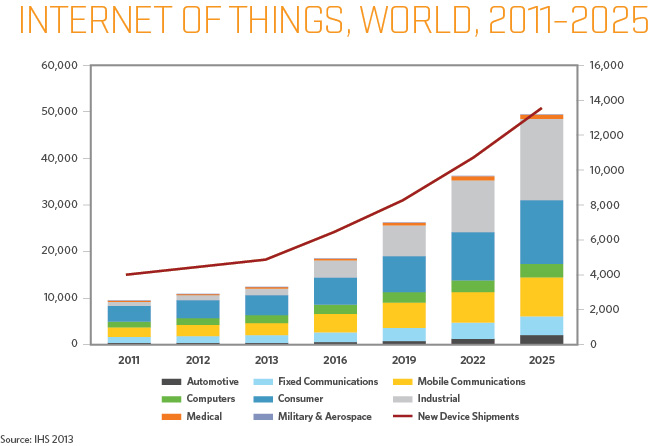
\includegraphics[scale=0.75]{graficoIot2011-2025}
\end{center}
\legend{Fonte: \citeauthor{ihs2013}, \citeyear{ihs2013} (Adaptado)}
\end{figure}

Tais dados se devem as consequências geradas pela emergência de tecnologias microeletrônicas, \textit{wireless} (\textit{Wi-fi}, \textit{Bluetooth} e \textit{ZigBee}), interfaces de comunicação móveis que se somaram as fixas já existentes e devido a formação de uma grande rede ubíqua capaz de conectar seres humanos com uma grande facilidade, possibilitando assim fornecer toda a base para a formação da IoT. \cite{santaella2013} 

\section{IoT}
\label{sec:iot}
No conceito de IoT um terceiro elemento foi inserido nas redes pervasivas que se possui hoje em dia, os objetos, sendo assim dentro da rede é possível se ter a comunicação entre humano-humano, humano-objeto e objeto-objeto, desta forma é possível ter humanos se comunicando normalmente como já acontecia anteriormente, humanos definindo comportamentos para os objetos e recebendo dados dos mesmos e objetos trocando informações entre si disponibilizando dados a humanos, dados estes, úteis para tomada de decisões ou até mesmo para facilitar atividades do dia a dia.\cite{santaella2013}

\begin{citacao}
Quando os objetos podem sentir o ambiente e se comunicar, eles se tornam ferramentas poderosas para entender coisas complexas e responder a elas com eficiência. Embora tais objetos inteligentes possam interagir com humanos, é mais provável que interajam ainda mais entre si automaticamente, sem intervenção humana atualizando-se com as tarefas do dia.\cite[p. 2]{presser2011}
\end{citacao}

Tais objetos podem ser considerados como tudo que está na rede e possui um endereçamento \textit{Internet Protocol} (IP), podendo interagir com outras interfaces endereçáveis dentro da mesma rede ou em outras através da internet, como mostra na figura \ref{fig:fluxogramaiot}.~\cite{ihs2013}

\begin{figure}[htb]
\caption{\label{fig:fluxogramaiot} Fluxograma da IoT}
\begin{center}
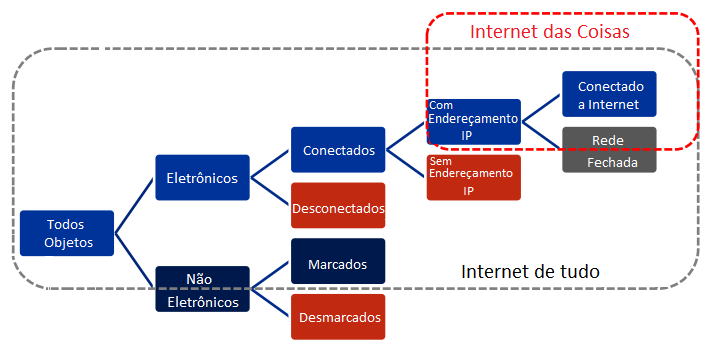
\includegraphics[scale=0.75]{fluxogramaiot}
\end{center}
\legend{Fonte: \citeauthor{ihs2013}, \citeyear{ihs2013} (Adaptado)} 
\end{figure}

Esses objetos podem ser um automóvel, uma geladeira, uma câmera, um sensor de temperatura, entre muitas outras interfaces, o que importa é que elas estão interligadas pela internet tomando ações de forma automática sem a intervenção humana. Pode-se citar o exemplo de um senhor que sofre de mal de Alzheimer e mora sozinho sendo que seus filhos não podem estar 24 horas por dia com ele, então os filhos decidem implantar sensores na casa do pai e pela vizinhança para que possam saber remotamente aonde ele está. Estes sensores estariam conectados a internet enviando dados para os filhos e emitindo alertas caso o pai saia de casa.\cite{presser2011}

Um outro exemplo de aplicação da IoT é apresentado na figura \ref{fig:exemploemergenciasiot}.

\begin{figure}[htb]
\caption{\label{fig:exemploemergenciasiot} Exemplo de aplicação da IoT}
\begin{center}
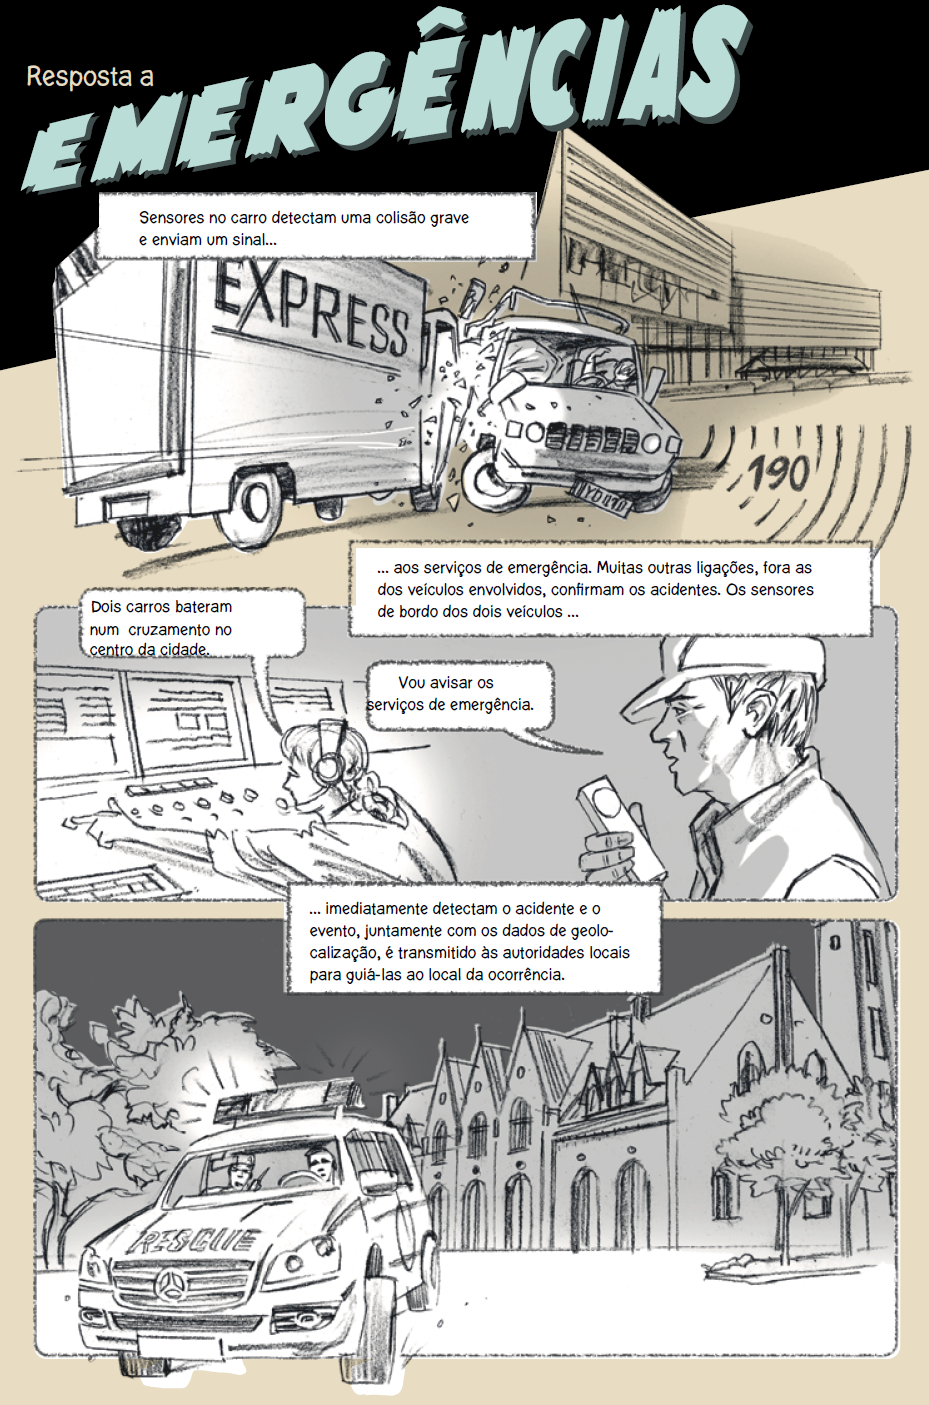
\includegraphics[scale=0.4]{exemploemergenciasiot}
\end{center}
\legend{Fonte: \citeauthor{presser2011}, \citeyear{presser2011} (Adaptado)} 
\end{figure}

Para que as aplicações de IoT tenha este tipo de comportamento é necessário que se tenha uma infraestrutura para dar suporte a esses objetos, ela pode ser estruturada de diferentes formas utilizando diversas tecnologias, mas de modo geral para o funcionamento de um sistema de IoT é necessário que se tenha os objetos conectados na internet ou a uma rede local, que envie e receba dados da infraestrutura (banco de dados ou armazenamento na nuvem) e os aplicativos que tem a função de gerenciar o sistema acessam e enviam os dados se comunicando diretamente com a infraestrutura, como é mostrado na figura~\ref{fig:estruturaiot}~\cite{ihs2013}

\begin{figure}[htb]
\caption{\label{fig:estruturaiot} Estrutura de um sistema de IoT}
\begin{center}
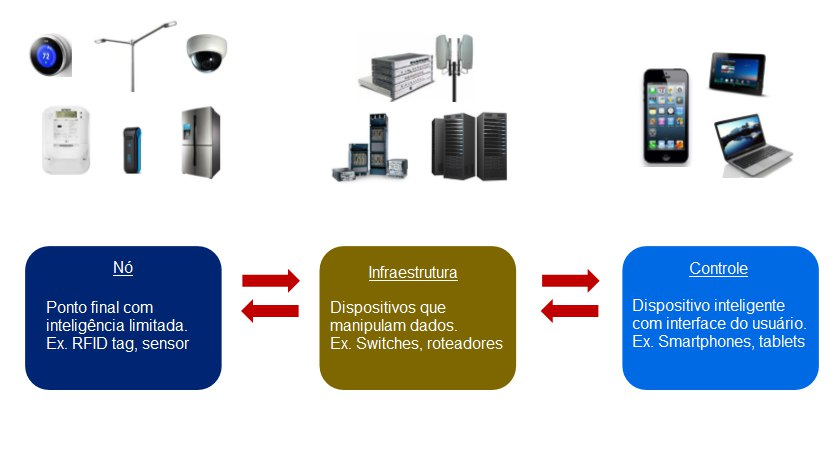
\includegraphics[scale=0.65]{estruturaiot}
\end{center}
\legend{Fonte: \citeauthor{ihs2013}, \citeyear{ihs2013} (Adaptado)} 
\end{figure}

\section{Cidades Inteligentes}
\label{sec:smartcities}
Com o grande crescimento da população como é possível ver na figura~\ref{fig:crescimentopopulacional}, as cidades também vem crescendo, mas de forma desordenada e desigual, causando problemas como o esgotamento de recursos, aumento da desigualdade social, aumento das áreas de favela, sem contar o caos com relação a locomoção dentro das cidades. Diante deste cenário criou-se o conceito de Cidades Inteligentes (\textit{Smart Cities}), que tem a finalidade de reinventar as cidades, ou seja reestruturá-las, a fim de que não haja desperdícios, tornando-a uma cidade sustentável e que a cidade seja organizada da melhor forma possível, trazendo uma melhor qualidade de vida aos cidadãos que nela vivem.\cite{leite2012cidades}

\begin{figure}[!h]
\caption{\label{fig:crescimentopopulacional} Impacto populacional}
\begin{center}
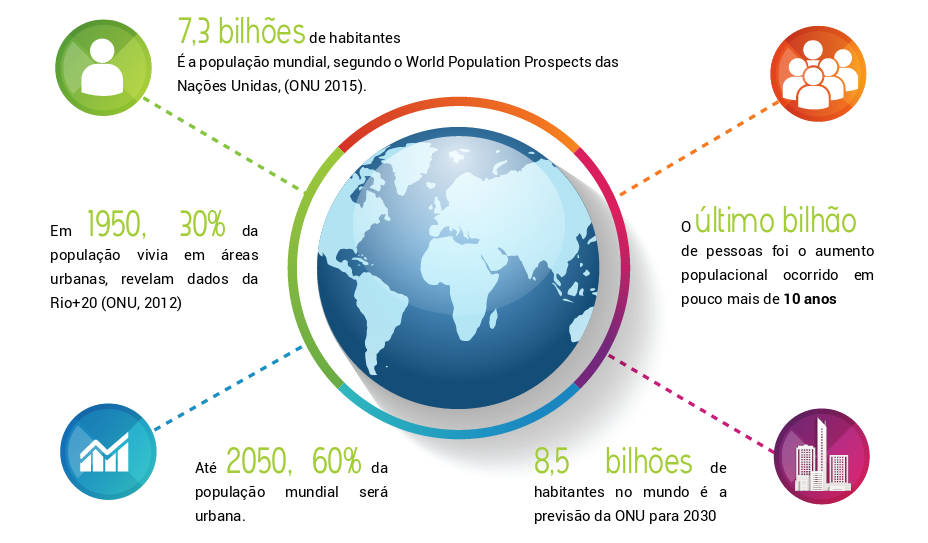
\includegraphics[scale=0.5]{crescimentopopulacional}
\end{center}
\legend{Fonte: \citeauthor{revistavia}, \citeyear{revistavia}} 
\end{figure}

Para tal reestruturação das cidades, transformando-as em Cidades Inteligentes, espera-se contar com o auxílio da área de Tecnologia da Informação e Comunicação (TIC), ou seja, boa parte das mudanças nas cidades se deverá pelo uso da tecnologia, mais especificamente pelas tecnologias de IoT. Elas poderão ajudar na redução de gases poluentes, redução na quantidade de lixo gerado pela população, redução do uso de recursos naturais, melhora da locomoção e segurança dentro das cidades, entre outras melhorias.\cite{leite2012cidades} 

\begin{citacao}
As maiores metrópoles do mundo têm adotado objetivos de tráfego e mobilidade para solucionar ou mitigar o problema de congestionamento com soluções de cidades inteligentes ativadas por Internet das Coisas (IoT), mas a mobilidade urbana não para em uma escolha contínua que consiste em se mover de A até B.~\cite[p. 1]{smartcities2017}.
\end{citacao}

\subsection{Mobilidade Urbana}
\label{subsec:mobilidadeurbana}
Dentro do conceito de Cidades Inteligentes, a mobilidade urbana se deve grande atenção, pois no século XXI ela tem se tornado um desafio a ser resolvido dentro das grandes cidades, pois o crescente número de veículos particulares causa um inchaço no trânsito, dificultando assim a locomoção, principalmente em grandes centros urbanos~\cite{gonccalomodelo}. Desta forma dentro de uma Cidade Inteligente a tecnologia pode ser aplicada para solucionar ou ao menos ser um paliativo aos problemas existentes, tecnologia esta que poderia atuar diretamente no trânsito, implantada através de \textit{smartphones} ou nos próprios carros, a fim de evitar acidentes, melhorar o fluxo, indicar rotas mais rápidas atuando diretamente na redução de gases poluentes e trazer maior facilidade aos motoristas.~\cite{gonccalomodelo}

\subsection{Saúde}
\label{subsec:saude}
Outro setor que se deve bastante atenção é o da saúde, pois é a necessidade básica da população, e infelizmente ela é muito precária nos dias de hoje, por diversos motivos principalmente os governamentais, mas através da tecnologia é possível que se mude este contexto. Com o uso de IoT é possível se criar aplicações na área da saúde que venha auxiliar no tratamento de doenças, cuidados com os pacientes, monitoramento e diagnósticos, transferência dos dados e colaboração, cadeiras de rodas inteligentes, Unidades de emergência conectadas, veículos de resposta, e hospitais, dentre tantas outras utilidades.~\cite{convergenciadigital}

Na área da saúde um grande desafio a se vencer é a de confiabilidade nos dados obtidos, pois um dado errado ou algo que se perca durante a transmissão pode representar a vida ou a morte de uma pessoa, visto que no futuro o uso de IoT na saúde será inevitável é necessário que se criem formas de manter esta tecnologia funcionando de forma segura e confiável.~\cite{convergenciadigital}

\section{V2V}
\label{sec:v2v}
Veiculo para Veiculo, ou V2V, habilita carros a se comunicarem entre eles em uma tentativa de avisar motoristas sobre potenciais acidentes ou colisões. A base da tecnologia é usar um onda de rádio de baixo alcance para permitir que os carros se comuniquem, podendo também que os carros enviem informações como localização, velocidade, direção, e também os estados dos freios, como mostra na figura~\ref{figsimulacao}.



\begin{figure}[!h]
\caption{\label{fig:simulacao} V2V simulação}
\begin{center}
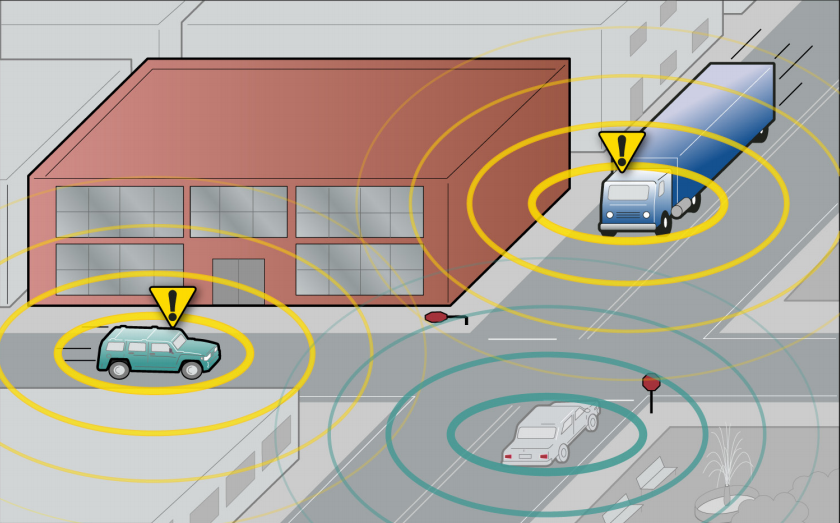
\includegraphics[scale=0.4]{v2v}
\end{center}
\legend{Fonte: \citeauthor{report2013}, \citeyear{report2013}} 
\end{figure}

\subsection{Regulamentação}
\label{subsec:regulamentacao}
Em dezembro de 2016 o Departamento de Transporte dos Estado Unidos (U.S. DOT) anunciou que esta trabalhando na regulamentação do uso da tecnologia em veículos de uso diário. O DOT diz que a tecnologia de rádio terá um alcance em média de 300 metros, e oferece um alcance maior que a abrangência de um radar ou câmera, em adição de não ser obstruídos por obstáculos ou outros veículos. O mesmo departamento acredita que a tecnologia poderá ser utilizada para avisar veículos sobre perigos eminentes particularmente quando se está em uma conversão ou realizando a troca de faixa. Adicionalmente, o departamento diz que os carros com sistemas automáticos de direção (ou até mesmo carros completamente autônomos) se beneficiaram das informações fornecidas pelo sistemas V2V.~\cite{usdot}

\section{V2I}
\label{sec:v2i}
Da mesma forma como acontece no caso do V2V, no paradigma de Veículo para Infraestrutura (V2I) os carros podem se comunicar, mas aqui a comunicação ocorre entre o carro e a infraestrutura, podendo receber instruções dela, assim como enviar instruções sobre as condições do veículo ou dados sobre o trânsito. A infraestrutura por sua vez, vem a ser as antenas que captam os dados do carro e os enviam para a nuvem, podendo usar estas informações transmitidas para se tomar decisões sobre o trânsito, analisar estatísticas, apontar trechos em que seja necessária a intervenção dos agentes de trânsito e trazer maior facilidade para o gerenciamento do mesmo.~\cite{howard2014}

Além da administração por parte dos agentes organizacionais, é possível que estes enviem mensagens para os carros a fim de alertar sobre algo á frente ou passar alguma informação relevante ao motorista, desta forma é possível notar as grandes vantagens trazidas por esse tipo de conexão que pode evitar acidentes e melhorar as condições do trânsito.~\cite{howard2014}

\subsection{Aplicação}
\label{subsec:aplicacao}
Como é apresentado em~\cite{tecmundo} hoje já é possível se ter exemplos da aplicação desta tecnologia, é o caso da empresa alemã Audi que está implantando nas próximas versões dos seus carros a tecnologia que ao parar em um semáforo inteligente, é exibido no painel do carro um temporizador indicando quanto tempo falta para abrir o semáforo, algo tido como não muito útil inicialmente, mas é só o começo do que há de vir, a ideia é avançar em busca de carros autônomos. 

O funcionamento deste sistema se dá pela comunicação do carro com as centrais de tráfego, instaladas nos semáforos, estas por sua vez se comunicam com os servidores, os quais enviam a informação que o veículo necessita, ao receber essas informações os veículos podem tomar ações, no caso de um carro autônomo (futuramente) ele poderia se preparar para uma parada no semáforo, trazendo maior economia de combustível.

Esta é uma tecnologia que tende a aumentar com o passar dos anos, pois no momento ainda é preciso que se reestruturem as cidades para que possa receber este tipo de tecnologia, como é o caso das centrais de tráfego, que atualmente não há este tipo de dispositivo instalado dentro das cidades, mas futuramente será algo necessário e que trará grandes benefícios a população podendo gerenciar o trânsito de forma inteligente evitando congestionamentos e gerenciando de forma mais eficiente o tempo dos semáforos.

\section{Funcionamento de Dispositivos de IoT}
\label{sec:dispositivosiot}
Quando se fala no uso de tecnologias IoT logo se pensa em sensores conectados na rede captando dados, sendo assim é preciso se detalhar o que são estes dispositivos e como funcionam.

\subsection{Sensores}
\label{subsec:sensores}
Sensor é o termo para designar um dispositivo sensível a algum tipo de energia do ambiente, podendo ela ser luminosa, térmica, cinética, relacionado a uma grandeza física como temperatura, pressão velocidade, corrente, aceleração, etc. Normalmente o sinal de saída de um sensor deve ser manipulado antes de sua utilização, geralmente através do uso de um amplificador, pois as tensões de saída após o dispositivo ser sensibilizado costumam ser baixas.~\cite{wendling2010}

\subsection{Transdutores}
\label{subsec:transdutores}
É o termo designado para se referenciar o dispositivo que transforma um tipo de energia em outra, trabalham geralmente junto com os sensores transformando o impulso elétrico vindo dos sensores em valores digitais úteis dentro de um sistema de IoT. Um exemplo de transdutor é o alto-falante que converte o impulso elétrico em movimento mecânico necessário para reproduzir o som.~\cite{wendling2010}


%\autoref{chap:cap1}
% ---
%\section{Aliquam vestibulum fringilla lorem}
%\lipsum[2]
%\subsection{Subsessão cap 1}
%\lipsum[2]
%\chapter{Capitulo Segundo}
%\lipsum[2]

\chapter{Sistemas de Big Data}
\label{chap:bigdata}
Explicar o conceito de Big Data, ferramentas dentro do trabalho que se utiliza para aplicá-la, mostrando juntamente a tecnologia que será empregada para o desenvolvimento.

\section{V2V}
\label{sec:v2v}
Apresentar a tecnologia \textit{Vehicle to Vehicle} (V2V), juntamente com seu uso dentro dentro do projeto e mostrar os pontos positivos do uso.

\section{V2I}
\label{sec:v2i}
Apresentar a integração do \textit{Vehicle to Infrastructure} (V2I) com o V2V, mostrar o que seria a infraestrutura para com a qual o veículo vai se comunicar e as tecnologias usadas para essa integração.

\section{Análise dos dados}
\label{sec:analisedados}
Mostrar como é feita uma análise de grande volume de dados em tempo real vinda do V2V e V2I, tecnologias empregadas, diversos tipos de dados como entrada.


 
\chapter{Especificações e Arquitetura do Sistema}
\label{chap:arquitetura}
Durante todo o desenvolvimento do sistema, buscou-se não se utilizar dos modelos de arquitetura comumente empregados neste tipo de aplicação, que trabalham com grandes volumes de dados, um dos motivos vem a ser pela grande complexidade encontrada ao se trabalhar com módulos Apache como o Hadoop Common, Hadoop Distributed File System (HDFS), Hadoop YARN e Hadoop MapReduce, os quais dependendo de suas aplicações acabam por gerar dependências de outras ferramentas como Cassandra, Spark, ZooKeeper, entre outras que se mostram apesar de robustas, muito complexas e com uma curva de aprendizagem alta demais para serem usadas de imediato.

Outro motivo de grande valor para o desenvolvimento de uma nova arquitetura tem sido a empregabilidade de novas ferramentas utilizadas no lado \textit{backend}, por assim dizer, relacionado a organização dentro dos servidores, conceitos de desenvolvimento e bancos de dados que tem ganhado força dentro do mercado e se mostradas bem aplicáveis em projetos com grandes volumes de dados e alta disponibilidade, além de possuir uma baixa curva de aprendizagem, se comparadas com as tecnologias tradicionais.

\section{Micro Serviços}
\label{sec:microserviços}
Os Micros Serviços tem se tornado um padrão de projeto muito utilizado em aplicações de multiplataforma, pois através deste padrão este tipo de aplicação tem se tornado mais fácil de se desenvolver, demandando menos tempo. A ideia do padrão de Micro Serviços é desenvolver pequenos serviços autônomos que trabalham juntos, ou seja, um serviço possui uma única responsabilidade bem definida, mas para o funcionamento da aplicação por completa é necessário o uso de todos os serviços disponíveis dentro do domínio da aplicação. Sendo assim, um serviço pode ser um \textit{endpoint} de uma \textit{Application Programming Interface} (API), que pode retornar informações como todos os dados de uma tabela.~\cite{newman2015building}

\section{CQRS}
O \textit{Command Query Responsibility Segregation} (CQRS) é um padrão de desenvolvimento que descreve como separar as operações de leitura e escrita em diferentes modelos, sendo que para a leitura é utilizada a \textit{Query model} e para outros comandos como atualização e inserção de dados é utilizado o \textit{Command Model}, os quais compartilham da mesma base de dados, como mostra a figura \ref{fig:cqrs}.

\begin{figure}[!h]
\caption{\label{fig:cqrs} Arquitetura CQRS}
\begin{center}
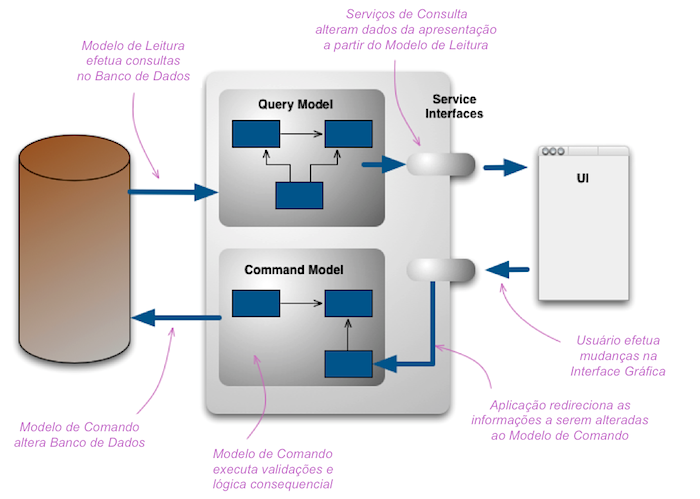
\includegraphics[scale=0.4]{cqrs}
\end{center}
\legend{Fonte: \citeauthor{cqrs}, \citeyear{cqrs}} 
\end{figure}

Este padrão foi desenvolvido tendo em vista que ao se criar novas regras de leitura e escrita, novas formas de representação das informações são criadas, o que já não faz mais sentido manter em um único modelo quando se fala em responsabilidade única, este é um padrão que adiciona grande complexidade ao projeto, portanto só deve ser utilizado caso as regras empregadas na leitura e escrita passem a ser complexas, não havendo um padrão fixo para todos os casos, é necessário adaptá-la ao problema que se deseja resolver.~\cite{cqrs}

\section{Docker Engine}
\label{sec:docker}
O Docker é uma plataforma aberta criada com o intuito de tornar mais ágil o desenvolvimento, implantação e execução de aplicações em ambientes isolados, além de ser multiplataforma, tudo isso através do conceito de conteinerização e imagens, em que numa imagem se tem todos os arquivos necessários para a criação de um contêiner, este por sua vez, possui a aplicação encapsulada  e funcionando.

Desta forma se tem uma grande flexibilidade para trabalhar com as aplicações, pois estas irão funcionar tanto em um notebook, quanto em um mainframe. Este conceito de contêiner se assimila ao processo de criação de máquinas virtuais, onde se tem todo o sistema operacional virtualizado, já o Docker realiza uma virtualização á nível do sistema operacional, mantendo um único kernel no \textit{host} executando processos (contêineres) de forma isolada, isso é possível através do uso de \textit{namespaces}, fazendo com que um processo só tenha acesso a recursos de outro se isso for explicitamente configurado na criação dos ambientes. Para que não ocorra a exaustão de recursos no \textit{host}, o Docker se utiliza de \textit{cgroups} do kernel, responsável por criar limites de hardware para os processos, evitando o uso exagerado de recursos por apenas um processo. A figura \ref{fig:arqdocker} apresenta a organização a nível de sistema operacional de um \textit{host} utilizando Docker.~\cite{docker}

\begin{figure}[!h]
\caption{\label{fig:arqdocker} Arquitetura Docker}
\begin{center}
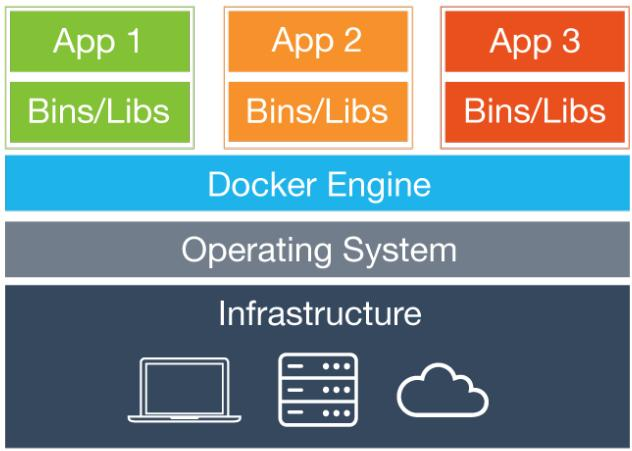
\includegraphics[scale=0.3]{arqdocker}
\end{center}
\legend{Fonte: \citeauthor{docker}, \citeyear{docker}} 
\end{figure}

O Docker tem ganhado fama no mercado, principalmente pelos profissionais de infraestrutura, pois ele tem facilitado o trabalho destas pessoas, fazendo com que elas economizem tempo para realizar a instalação de um software, não necessitando mais se preocupar com todas as dependências e ferramentas necessárias para o funcionamento do software, basta apenas se utilizar uma imagem da aplicação e transformá-la em um contêiner em qualquer ambiente que se esteja. Comumente o Docker não é utilizado isoladamente, pois o que traz a ele grande facilidade ao se trabalhar com contêineres é a junção de todas as suas ferramentas, as quais serão descritas a seguir.~\cite{docker}

\subsection{Docker Compose}
Com o aumento da complexidade do ambiente em que se está hospedada a aplicação, surgem as necessidades de se criar mais contêineres, tornando o seu gerenciamento um tanto quanto complicado, é neste cenário que se aplica o Docker Compose, uma ferramenta que trabalha juntamente com o Docker, ele se caracteriza por definir e executar múltiplos contêineres, pois através do uso de um arquivo que descreve todos os contêineres e configurações necessárias para o funcionamento de uma aplicação por completa, o Docker Compose tem a capacidade de criá-los, reiniciá-los e desligá-los quando necessário, facilitando assim o uso de contêineres.~\cite{docker}

\subsection{Docker Swarm}
Como visto até aqui, Docker Engine é o responsável pela arquitetura de criar e manter em funcionamento os contêineres, além de armazenar as imagens, o Docker Compose leva a responsabilidade da criação e remoção de múltiplos contêineres, facilitando o gerenciamento destes, por fim se tem o Docker Swarm a qual tem a função de gerenciar o \textit{cluster} de contêineres, ele pode ser considerado como um orquestrador de contêineres como mostra a figura \ref{fig:dockerswarm}, especificando quais máquinas e contêineres farão parte deste \textit{cluster}, sendo que muitos destes contêineres podem terem sidos criados a partir de um Docker Compose.   

\begin{figure}[!h]
\caption{\label{fig:dockerswarm} Docker Swarm}
\begin{center}
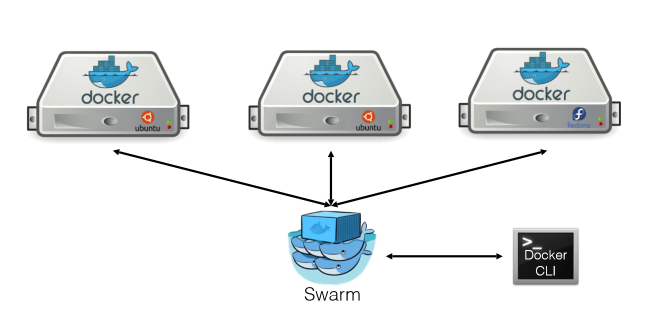
\includegraphics[scale=0.5]{dockerswarm}
\end{center}
\legend{Fonte: \citeauthor{dockerswarm}, \citeyear{dockerswarm}} 
\end{figure}


É o Docker Swarm que aplica todo o conceito de escalabilidade à aplicação conteinerizada, pois ela tem a capacidade de criar novas réplicas de contêineres de acordo com a necessidade, ou até os limites pré estabelecidos, é ele também que aplica o conceito de distribuição de cargas entre os contêineres que estão em funcionamento, podendo estes estarem na mesma máquina ou não, no caso de estarem em outra máquina o gerenciamento do Docker Swarm só é possível através da troca de \textit{tokens} entre elas formando um \textit{cluster} com contêineres homogêneos ou heterogêneos. É desta forma que é criado todo o ecossistema da arquitetura Docker, como pode ser visto na figura \ref{fig:ecossistemadocker}.~\cite{dockerswarm}  

\begin{figure}[!h]
\caption{\label{fig:ecossistemadocker} Ecossistema Docker}
\begin{center}
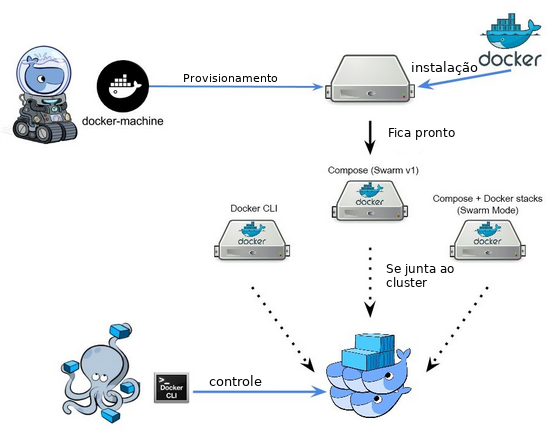
\includegraphics[scale=0.5]{ecossistemadocker}
\end{center}
\legend{Fonte: \citeauthor{dockerswarm}, \citeyear{dockerswarm}} 
\end{figure}

\section{Redis}
\label{sec:redis}
Redis é um banco de dados No-SQL destinado ao armazenamento em memória de dados no tipo chave-valor, utilizado para manter cache das aplicações, nesse cache podem ser armazenados \textit{hashs}, \textit{strings}, \textit{bitmaps}, listas e \textit{Hyperloglogs}, estes dados tem uma data de expiração após serem persistidos no Redis, por ser um banco de dados em memória, as ações de escrita e leitura se tornam mais rápidas do que uma leitura ou escrita em disco, dando maior \textit{performance} ás aplicações nas quais ele é implantado.~\cite{da2015redis}

\section{Clojure}
Apresentada ao público em 2007 ela foi desenvolvida visando a construção de aplicações multitarefa, aproveitando os recursos da \textit{Java Virtual Machine} (JVM), mas diferente do Java em que se escreve códigos orientado a objetos, em Clojure se tem códigos escritos em linguagem funcional, em que cada função é especializada em sua tarefa, sendo que a resolução de problemas se dá pela integração destas funções.

Algo que faz Clojure uma linguagem diferente das outras é que valores são imutáveis, isso resolve o problema que se tem de compartilhamento de memória quando usada várias \textit{threads}, outra funcionalidade interessante é a criação de macros, que é o equivalente a criar novas funcionalidades dentro da linguagem, algo muito útil para adequar a linguagem ao problema a ser solucionado. Além de tudo assim como o Ruby possuí o gerenciador de pacotes rake e o Java o Maven, Clojure possui o Leiningen, que gerencia os pacotes necessários para o seu funcionamento, além de disponibilizar um \textit{prompt} de comando para teste de trechos de código, similar ao pip do Python.~\cite{hickey2010clojure}

\section{Kafka}
O Kafka se caracteriza por ser uma central de mensagens distribuídas, em que todas as informações passam por ele antes de alimentarem um banco de dados, Data Warehouse ou algum outro sistema de análise de dados, dentre as suas vantagens estão a sua rapidez, alta escalabilidade e redundância, permite uma grande quantidade de conexões persistentes dos usuários , além de apresentar uma grande resiliência tendo a capacidade de se recuperar após a ocorrência de falhas. Desta forma o Kafka se torna ideal para comunicação e integração de componentes em sistemas de larga escala.

Seu funcionamento se dá através de partições sobre tópicos diferentes (como se fossem mensagens relacionadas a cada assunto, ou ainda pode-se comparar as tabelas de um banco relacional) que podem estar em diferentes máquinas, estas partições armazenam uma fila de mensagens, tendo cada uma delas um número identificador imutável que segue a ordem da fila, um consumidor dessa fila de mensagens tem a possibilidade de ler qualquer mensagem que esteja na fila através o seu identificador, um consumidor também pode consumir mensagens de diversas partições como mostra na figura \ref{fig:kafkatopicos}. As mensagens que chegam ao Kafka ficam armazenadas por um período de tempo configurável, não possuindo algo que informe se a mensagem foi lida ou não, apenas mantém pelo período estabelecido, caso o período seja menor ao período em que será feita a leitura pelo consumidor, essa mensagem será perdida

\begin{figure}[!h]
\caption{\label{fig:kafkatopicos} Partições do Kafka}
\begin{center}
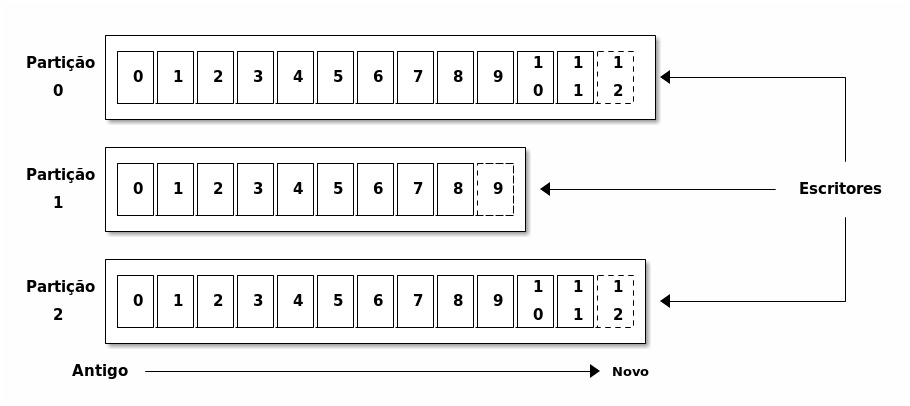
\includegraphics[scale=0.7]{kafkatopicos}
\end{center}
\legend{Fonte: \citeauthor{kafka}, \citeyear{kafka}} 
\end{figure}

Além da organização das mensagens dentro de partições, se tem ainda a organização de partições dentro de \textit{brokers}, onde se tem partições  chamadas de líderes e réplicas, no processo de produção de mensagens como apresentado na figura \ref{fig:kafkaproducao} o produtor escreve na partição líder, esta então gera cópia nas partições réplicas que podem estar em outros \textit{brokers} e em outras máquinas, desta forma se mantêm a consistência das mensagens e um alto nível de paralelismo, pois no processo de leitura o consumidor faz uma requisição para ler e a partição que está disponível retorna a mensagem para ele.~\cite{kafka}

\begin{figure}[!h]
\caption{\label{fig:kafkaproducao} Processo de escrita do Kafka}
\begin{center}
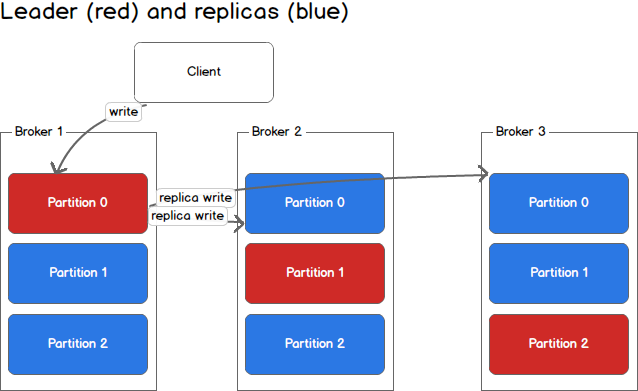
\includegraphics[scale=0.5]{kafkaproducao}
\end{center}
\legend{Fonte: \citeauthor{kafka}, \citeyear{kafka}} 
\end{figure}

\section{MongoDB}
MongoDB é um banco de dados orientado a documento, organizado em coleções de dados, aos quais se permitem operações de leitura e escrita, substituindo o conceito de linhas dos bancos relacionais por documentos, uma das grandes vantagens deste modelo é a fácil escalabilidade possível de se empregar, além da grande flexibilidade que se tem, pois não são pré-definidos identificadores, tamanhos ou tipos de dados para os documentos armazenados.

Dentre as funcionalidades dele se destacam a indexação através de texto o que mantêm uma boa \textit{performance} na execução de \textit{queries}, agregações complexas através de pedaços mais simples de código, tipos especiais de coleções suportando tamanhos fixos, suporta também o armazenamento de grandes documentos além de metadados. Seu funcionamento difere aos de bancos relacionais por não possibilitar as funções como \textit{joins}, ou seja, para utilizá-la é preciso que se armazene dados completos em um único objeto, pois quando se tenta utilizá-lo similar a um banco relacional toda a \textit{performance} da ferramenta quanto as buscas se perde.~\cite{chodorow2013mongodb}

\section{Datomic}
Assim como o MongoDB ele é um banco de dados não relacional, mas com um conceito diferente, adaptado para as novas demandas de serviços em nuvem com arquitetura \textit{Software as a Service} (SaaS), Datomic é um banco de dados orientado a fatos, com o grande diferencial de que dados nele persistidos se tornam imutáveis, isto não significa que não se pode alterar dados, mas o que acontece é um versionamento dos dados, desta forma é possível se ter um histórico do objeto persistido com todas as alterações já realizadas sendo a última versão o dado de maior veracidade.  

Possui como características separação dos conceitos de leitura e escrita, forte garantia transacional na escrita, noções de imutabilidade expressas por bases de dados estritamente incrementais, utiliza para as consultas de dados a linguagem Datalog, como é mostrado um exemplo da linguagem na figura \ref{fig:datalog} que é estruturada baseada em lógica permitindo consultas complexas incluindo \textit{joins} inferidos.~\cite{datomic} 

\begin{figure}[!h]
\caption{\label{fig:datalog} Exemplo da linguagem Datalog}
\begin{center}
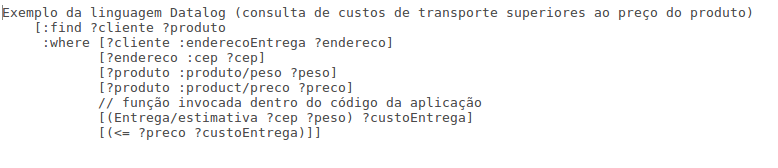
\includegraphics[scale=0.6]{datalog}
\end{center}
\legend{Fonte: \citeauthor{datomic}, \citeyear{datomic}} 
\end{figure}

\section{Locust}
Locust é uma ferramenta \textit{open source} desenvolvida em Python que visa realizar testes de carga e \textit{stress} simulando conexões de usuários reais, para estes testes podem ser usados máquinas \textit{slaves} tendo um teste de forma distribuída, a configuração é feita através de um \textit{script} em Python também, onde são definidas as URLs a serem testadas, e por meio de uma interface gráfica WEB é possível configurar a quantidade de usuários a serem simulados, quantidade de requisições a serem feitas, além de apresentar gráficos estatísticos sobre os testes.~\cite{locust}

\section{Arquitetura do Sistema}
Durante o desenvolvimento do projeto buscou-se utilizar do padrão de micro serviços, com cada um deles encapsulado dentro de um contêiner com responsabilidade única, sendo utilizado um arquivo Docker Compose para sua criação, e o Docker Swarm para realizar todo o gerenciamento de carga da aplicação. A escolha de se utilizar micro serviços conteinerizados se deu pela grande facilidade com que se pode criar, remover e escalar toda a aplicação, por exemplo, se em algum momento um serviço em específico está sendo mais utilizado que os demais, automaticamente podem ser criadas réplicas deste serviço para atender as demandas.~\cite{dockerswarm}

Utilizou-se também do padrão CQRS para a execução das operações de escrita e leitura, utilizado por se tratar de um sistema ao qual as regras tendem a aumentar sua complexidade, e assim estando no padrão CQRS a aplicação já estará pronta para suportar estas demandas. Para conhecimento da arquitetura por completa será analisado o fluxo de dados seguido pelo dado objeto a seguir, o qual é criado assim que um carro é ligado e faz uma requisição para se conectar a infraestrutura (iniciar uma nova sessão) no serviço de \textit{Command}:
\begin{lstlisting}
{
	"hd-id": "abcd1234",
	"model": "zyz",
	"brand": "123"
}
\end{lstlisting}

\subsection{\textit{Command}}
Operações de leitura, escrita e remoção passam por este serviço, escrito em Clojure devido ao seu alto paralelismo, que validará com as regras de negócio as informações recebidas e se passarem por esta fase, as informações serão inseridas em forma de texto na fila de mensagens do Kafka para serem inseridos no banco de dados juntamente com um identificador da sessão criada para este carro, o dado enviado ao Kafka é apresentado a baixo:
\begin{lstlisting}
{
	"command": "create_session",
	"session-id": "{uuid}",
	"hd-id": "abcd1234",
	"model": "zyz",
	"brand": "123"
}
\end{lstlisting}

\subsection{\textit{Worker}}
Após a inserção da mensagem na fila do Kafka um outro serviço chamado de \textit{Worker} que monitora se existem mensagens a serem lidas no Kafka, irá ler esta mensagem e salvá-la banco de dados, neste caso por ser uma informação apenas de sessão será salvo apenas no MongoDB, mas para o caso de um novo cadastro de veículo ou alteração do mesmo, este serviço salvaria primeiramente no Datomic, o qual armazena dados históricos e posteriormente no MongoDB, o qual terá a informação imediata sobre o veículo, juntamente com esta informação de sessão o serviço de \textit{tracking} estará atualizando dados referentes a localização do veículo, como pode ser visto no objeto persistido no MongoDB apresentado a seguir: 
\begin{lstlisting}
{
	"session-id": "{uuid}",
	"hd-id": "abcd1234",
	"model": "zyz",
	"brand": "123",
	"location": {"x": 46.121, "y": 12.0213},
	"gas-lvl": 74
}
\end{lstlisting}

Esta estratégia de se salvar em dois bancos de dados faz com que Datomic fique armazenados todas as informações relevantes para se manter um histórico do veículo, mantendo a veracidade de dados sobre a entidade, já no MongoDB se tem os dados em tempo real e como pôde ser visto a grande vantagem do banco não relacional está na rapidez com que esse dado poderá ser buscado, pois em um banco relacional provavelmente se teria uma tabela para localizações e uma para dados do veículo, necessitando de funções de agregação de dados para se ter o objeto completo, desta forma, no banco não relacional todas as informações já estão agrupadas, se ganhando muito em velocidade.

\subsection{\textit{Tracking}}
O serviço de \textit{tracking} é o responsável por receber informações do veículo, como posição e velocidade, dentre algumas informações sobre o estado do carro, e colocá-las na fila de mensagens do Kafka, para serem inseridos pelo serviço \textit{worker} no MongoDB, juntamente com as informações de sessão do carro. 

\subsection{\textit{Query}}
Finalizado o processo de inserção de dados, o processo de leitura se dá pelo serviço de \textit{query}, o qual recebe a requisição do usuário e busca dados diretamente no MongoDB retornando assim as informações requisitadas, consultas realizadas no Datomic estão relacionadas com as análise de dados do Big Data, pois é lá que se formará a grande massa de dados possíveis de serem analisadas com o decorrer do tempo.

\subsection{Interface do Usuário}
Esta vem a ser o dispositivo implantado no carro que tem a função de se ligar aos sensores do carro, a fim de mandá-las para a infraestrutura, juntamente com a localização instantânea do veículo. Esta interface não é contemplada pelo projeto, mas é essencial para o seu funcionamento prático.

\subsection{Visão Geral}
De forma geral se tem um fluxo de dados para inserção como visto na figura \ref{fig:insert} e o fluxo de dados para leituras apresentadas na figura \ref{fig:select}, a estrutura geral de toda arquitetura é representada na figura \ref{fig:estruturageral}.

\begin{figure}[!h]
\caption{\label{fig:insert} Fluxo de dados para inserção}
\begin{center}
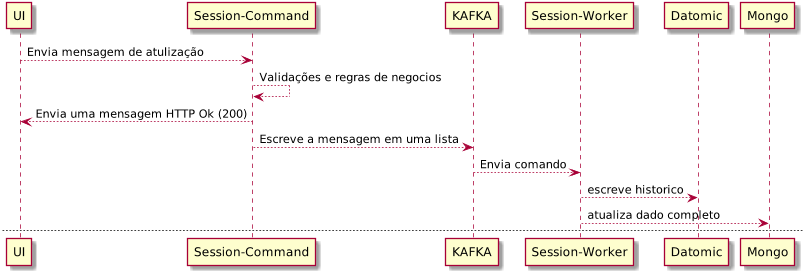
\includegraphics[scale=0.5]{insert}
\end{center}
%\legend{Fonte: SOUZA} 
\end{figure}

\begin{figure}[!h]
\caption{\label{fig:select} Fluxo de dados para leitura}
\begin{center}
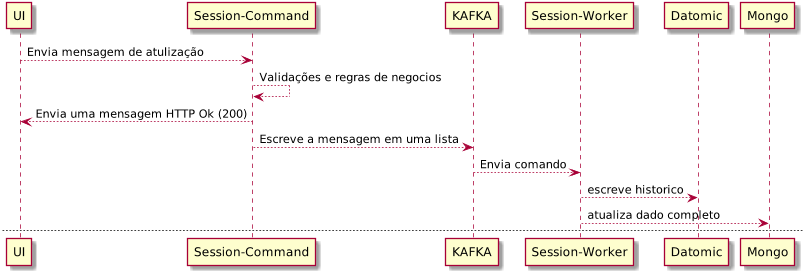
\includegraphics[scale=0.4]{select}
\end{center}
%\legend{Fonte: COELHO} 
\end{figure}

\begin{figure}[!h]
\caption{\label{fig:estruturageral} Estrutura Geral da Arquitetura}
\begin{center}
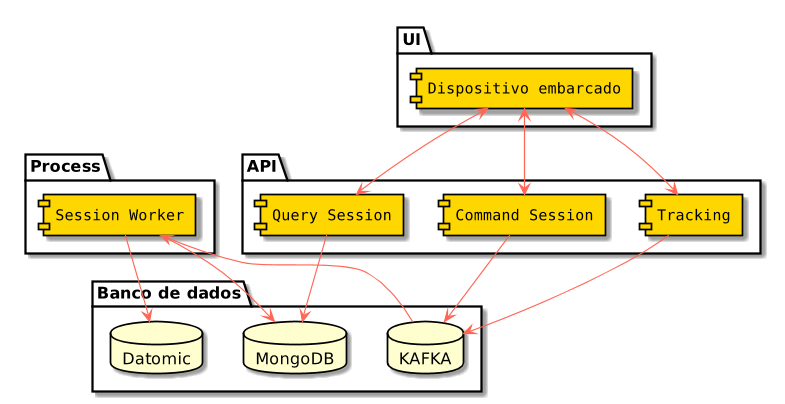
\includegraphics[scale=0.5]{estruturageral}
\end{center}
%\legend{Fonte: COELHO} 
\end{figure}

\chapter{Resultados}
\label{chap:analiseresultados}
Inicialmente para criação da arquitetura especificada na seção \ref{chap:arquitetura}, criou-se o serviço de \textit{Command}, o qual é a porta de entrada entre a interface de usuário e a arquitetura, este serviço tem a função de receber os dados da interface, validá-los e inserir na fila do Kafka, é através dela que um carro terá a sua sessão criada (\textit{Command Session}), ou informará dados sobre a localização (\textit{Command Track}), ou ainda informações de alerta (\textit{Command Warning}), para isso, como pode ser observado no apêndice \ref{ap:sessioncommand}, se tem as validações para cada um dos modelos de dados, no caso das informações referentes a sessão se tem informações sobre a marca, modelo, placa e proprietário, para o modelo de localização o identificador da sessão, nível de combustível, latitude, longitude e velocidade, para o modelo de alertas o identificador da sessão e o alerta emitido, todos estes dados são manipulados e recebidos no formato \textit{JavaScript Object Notation} (JSON) por questões de velocidade e uso de memória. Ainda no apêndice  \ref{ap:sessioncommand} é apresentado todos os comandos de envio para a fila do Kafka de cada um dos modelos de dados.

Seguindo a arquitetura, tornou-se necessário a configuração da fila de mensagens (Kafka), a qual tem a função de armazenar uma informação por um determinado tempo até que ela seja consumida por algum outro serviço. Para isso utilizou-se imagens Docker vindas de repositórios oficiais, sendo necessário um contêiner Kafka Zookeeper que é o sistema responsável por gerenciar os \textit{brokers} do Kafka, e o Kafka Broker que são os \textit{brokers}, onde ficam armazenados os tópicos, cada um funcionando em um contêiner separado.

O próximo passo que se tem dentro da arquitetura é a criação do micro serviço \textit{Worker}, o qual tem a finalidade de ler dados da fila de mensagens e armazená-las nos bancos de dados, para isso este micro serviço foi criado em Clojure, contendo a conexão com o Kafka, além das conexões com os bancos de dados MongoDB e Datomic, o apêndice \ref{ap:sessionworker} mostra a retirada de dados da fila de mensagens e gravação dos dados nos bancos MongoDB e Datomic de acordo com o tipo de informação contida na mensagem.

Por fim foram configurados os bancos de dados, os quais armazenam os dados vindos dos serviços de \textit{Workers} e os mantém para consultas instantâneas no caso do MongoDB, ou consultas históricas no caso do Datomic. Para os dois bancos de dados utilizou-se de imagens Docker oficiais com a base de dados armazenadas no \textit{host}, para que os dados fiquem disponíveis para todos os contêineres, mesmo quando estes sejam replicados.

Tendo os dados armazenados, para o processo de leitura destes dados criou-se o micro serviço \textit{Command Query} também em Clojure, o qual tem a função de ler os dados inseridos no MongoDB ou no Datomic, sem passar pela fila de mensagens diretamente ele realiza a função de busca de dado desejado diretamente no banco de dados que se deseja, retornando para o usuário que requisitou esta informação a ser exibida no painel do carro.

Todos os micro serviços  utilizados dentro da arquitetura apresentam-se encapsulados dentro de contêineres, estes porém, possuem a base inicial vinda de uma imagem Docker oficial, no caso dos micro serviços utilizou-se a imagem Java com \textit{Java SE Runtime Environment} (JRE) em sua versão 8, sendo assim, as alterações e configurações para o ambiente desejado se fizeram através do Dockerfile, que ao ser construído gera uma nova imagem com as alterações nele contidos, e para criação do contêiner basta especificar que a imagem a ser usada será esta nova imagem.



\section{Testes de Sistema}
\label{sec:testessistema}
Montada a arquitetura especificada na seção \ref{chap:arquitetura}, iniciou-se o processo de inserção de dados nesta estrutura através do conceito de \textit{Mockup}, o qual simula funcionalidades do sistema para que estas possam ser testadas de forma independente, sendo assim, dentro desta arquitetura os objetos \textit{mock} foram os carros e unidades de emergência, os quais tiveram seu comportamento simulado via \textit{software}, a fim de validar o armazenamento e fluxo de dados na arquitetura.

O \textit{Mockup} realizou-se por meio de um micro serviço escrito em Clojure, o qual cria uma quantidade de conexões pré-estabelecidas com o micro serviço \textit{Session Command} e envia dados fictícios sobre localização, nível de combustível e alertas em cada conexão criada, esses dados passam a serem inseridos na fila do Kafka após terem as informações validadas pelo \textit{Session Command}, desta forma o micro serviço \textit{Session Worker} retira da fila e popula os bancos de dados Datomic ou MongoDB

\section{Testes de Aceitação}
\label{sec:testesaceitacao}
Análise dos resultados obtidos e analisar o benefício do usuário utilizador do sistema, analisar se seria aprovado pelo mesmo e pelos agentes sociais.

\section{Discussão de Resultados}
\label{sec:discussãoresultados}
Aqui se apresenta os resultados gerais, estatísticos, apresentando os principais pontos positivos e negativos do trabalho baseados nos dados analisados.

% ----------------------------------------------------------
% Finaliza a parte no bookmark do PDF
% para que se inicie o bookmark na raiz
% e adiciona espaço de parte no Sumário
% ----------------------------------------------------------
\phantompart

% ---
% Conclusão
% ---
\chapter{Conclusão}
\label{chap:conclusao}
O desenvolvimento do presente sistema possibilitou a criação de uma nova arquitetura para um sistema de \textit{Big Data}, pois como apresentado, o sistema leva características dos 5Vs presente presente neste tipo de arquitetura, contendo um grande volume de dados, pois o sistema quando em operação gera uma massa de dados gigantesca vinda das milhares de conexões que se tem com todos os carros que estão no trânsito, as requisições são atendidas com uma alta velocidade, pois neste tipo de aplicação se torna inadmissível a demora na obtenção de uma resposta, e mesmo com o grande volume de requisições o sistema consegue manter a veracidade dos dados, tudo isso sem um alto consumo de recursos de \textit{hardware}, já que este pode não estar concentrado em um único ponto, mas sim distribuído entre várias máquinas. Sendo assim, a arquitetura e o sistema proposto realmente atendem os resultados esperados com relação a urgências no trânsito e prova que poderia ser utilizado em outros estudos de caso.

Outro ponto que se esperava com a arquitetura era a fácil utilização da mesma, diferente do que ocorre com as ferramentas tradicionais com relação a instalação e uso propriamente dito, a arquitetura especificada por possuir ferramentas dedicadas a instalação e gerenciamento das instâncias se apresenta mais simples e rápida de ser manipulada e através dos micro serviços que também podem ser chamados de \textit{Application Programming Interface} (API) quando analisado na visão da interface de usuário, a integração com outros sistemas os quais enviem ou consumam dados se torna fácil, mantendo a alta escalabilidade do sistema, tanto em relação a distribuição, como em relação aos dados armazenados.

Dentre as principais dificuldades durante a montagem da arquitetura especificada, está a dificuldade em se trabalhar com Clojure, apesar de todas as características e benefícios já mencionadas anteriormente, por ser uma linguagem recém lançada no mercado e não possuir uma comunidade ativa para a resolução de problemas encontrados com a linguagem, encontrar suporte e documentação para o desenvolvimento se tornou uma tarefa difícil, se fazendo necessário a análise puramente de \textit{logs}, que por muitas vezes não eram específicos da linguagem, mas sim da JVM, o que tornou mais difícil a obtenção de soluções, embora torne o aprendizado mais rico, este tipo de análise demanda maior tempo.

Em uma primeira fase do projeto ao invés de Kafka como fila de mensagens utilizou-se o Redis, apesar de se mostrar eficiente, limitava a questão de escalabilidade e distribuição do sistema, pois ele vem a ser uma fila simples sem replicação das filas como acontece no Kafka, desta forma ele foi substituído pelo Kafka que apesar de mais robusto também se apresentou mais complexo nas suas configurações, principalmente com relação ao encapsulamento em contêiner.

Como trabalho futuro para a arquitetura apresentada se tem o desenvolvimento da interface de usuário, que vem a ser o dispositivo embarcado presente nos carros, juntamente com a rede pela qual as informações trafegarão entre a infraestrutura e o veículo, para a escolha de ambas é necessário que se faça uma análise para a decisão de qual sistema de IoT deve ser utilizado, podendo se chegar ainda a conclusão de que a melhor forma seria o uso do celular do motorista conectado a rede 3G, pois a arquitetura permite comunicação com qualquer interface de usuário, provando mais uma vez a sua escalabilidade. 

Por apresentar uma causa nobre e escolha dos autores, todo o projeto está aberto em um repositório no GitHub (https://github.com/alexcvcoelho-gabrielgio) sob a licença GPL2, onde é possível encontrar todos os códigos desenvolvidos, configurações necessárias e \textit{links} de referência para as tecnologias, sendo assim, o trabalho fica aberto a possíveis colaboradores ajudarem a definir os próximos passos e direções a serem tomadas com o projeto.



% ----------------------------------------------------------
% ELEMENTOS PÓS-TEXTUAIS
% ----------------------------------------------------------
\postextual
% ----------------------------------------------------------

% ----------------------------------------------------------
% Referências bibliográficas
% ----------------------------------------------------------
\bibliography{pos-textuais/bibliografia}

% ----------------------------------------------------------
% Glossário
% ----------------------------------------------------------
%
% Consulte o manual da classe abntex2 para orientações sobre o glossário.
%
%\glossary

% ----------------------------------------------------------
% Apêndices
% ----------------------------------------------------------

% ---
% Inicia os apêndices
% ---

% ---
\begin{apendicesenv}

% Imprime uma página indicando o início dos apêndices
%\partapendices

% ----------------------------------------------------------
\chapter{\textit{Session Command}}

\begin{lstlisting}
(ns session-command.kafka.core
  (:require [kinsky.client :as client]
            [session-command.config :refer [env]]
            [clojure.core.async :as a]
            [jkkramer.verily :as v]))

(def s-validate (v/validations->fn [[:required [:brand :model :hd-id :command :uuid]]]))
(def t-validate (v/validations->fn [[:required [:session-id :gas-lvl :lat :long :vel]]]))
(def w-validate (v/validations->fn [[:required [:session-id :action]]]))

(mount.core/defstate conn
                     :start (client/producer {:bootstrap.servers (env :kafka)}
                                             (client/keyword-serializer)
                                             (client/edn-serializer))
                     :stop (client/close! conn))

(defn push-session [session]
  (if (s-validate session)
    (client/send! conn "session" :session session)
    {:error "Value can be null"}))

(defn push-warn [warn]
  (if (w-validate warn)
    (client/send! conn "warn-warn" :session warn)
    {:error "Value cannot be null"}))

(defn push-track [track]
  (if (t-validate track)
    (client/send! conn "track" :track track)
    {:error "value cannot be null"}))
\end{lstlisting}

% ----------------------------------------------------------
\chapter{\textit{Session Worker}}
\begin{lstlisting}
(ns session-worker.core
  (:gen-class)
  (:require [ext.kafka :as kf]
            [clojure.core.async :refer [go thread chan <!!]]
            [ext.router :as rt]
            [clojure.data.json :as json]
            [clojure.tools.logging :as log]))

(defn pull [item]
  (println (:command item) " " (:uuid item))
  (case (:command item)
    "create_session" (rt/save-session item)
    "warn" (rt/save-warn item)
    nil))

(defn loop-through [c]
  (loop [count 0]
    (try
      (println "LOOP" count)
      (kf/pop-session-async c)
      (doseq [i (<!! c)]
        (pull i))
      (catch Exception e
        (-> e print)))
    (recur (inc count))))

(defn -main [& args]
  (mount.core/start)
  (let [c (chan)]
    (loop-through c)))
\end{lstlisting}


\end{apendicesenv}

% ----------------------------------------------------------
% Anexos
% ----------------------------------------------------------

% ---
% Inicia os anexos
% ---
%\begin{anexosenv}

% Imprime uma página indicando o início dos anexos
%\partanexos

% ---
%\chapter{Morbi ultrices rutrum lorem.}
% ---
%\lipsum[30]

% ---
%\chapter{Cras non urna sed feugiat cum sociis natoque penatibus et magnis dis
%parturient montes nascetur ridiculus mus}
% ---

%\lipsum[31]

% ---
%\chapter{Fusce facilisis lacinia dui}
% ---

%\lipsum[32]

%\end{anexosenv}

%---------------------------------------------------------------------
% INDICE REMISSIVO
%---------------------------------------------------------------------
%\phantompart
\printindex
%---------------------------------------------------------------------

\end{document}
